%%% This file contains the second  report. It cannot be compiled on it's own.

%{{{ Versuch 2

\setcounter{section}{2}
\addsec{Versuch 2}
%{{{
Der Zweite Versuch beschäftigte sich mit Dioden und ihren Eigenschaften. Zum Messen verwendeten wir in diesem Versuch hauptsächlich das Oszilloskop. Ausserdem simulierten wir in diesem Versuch unsere Schaltungen zuvor mit pSpice \cite{spice}.
%}}}

%{{{
\subsection{Kennlinie einer pn-Diode (1N4148)}
In diesem Versuch wird die Kennlinie einer Standard-pn-Diode, 1N4148, ausgemessen. Die ermittelte Kennlinie ist im folgenden Diagramm dargestellt.
In diesem Versuch wird das Ohm'sche Gesetz an einem Widerstand nachgemessen.
Das Skript schlägt 2 verschiedene Möglichkeiten vor, wie die Messgeräte platziert werden könnten:
\begin{figure}[H]
	\centering
	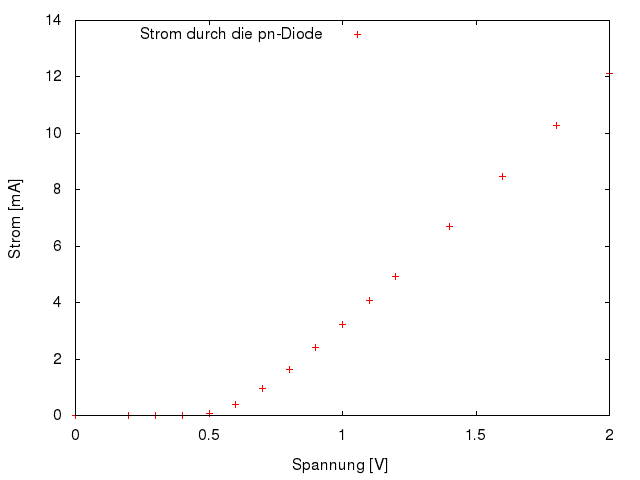
\includegraphics[width=\linewidth]{versuch2/versuch_2_1.png}
	\caption{Strom in Abhängigkeit der angelegten Spannung}
\end{figure}
Es zeigt sich schön, dass die Diode bei 0.5 V noch nicht leitet. Erst beim nächsten Messpunkt bei 0.6 V stellt sich ein nennenswerter Strom ein. Dies passt zu den erwarteten Werten von 6.2 V bis 0.72 V Vorwärtsspannung bei 5 mA, die das Datenblatt von NXP angibt.\\
So kann man den Widerstand berechnen. Es gilt: $\Delta U / \Delta I = R_Diode + R_Vorwiderstand$\\
Stellt man dies um, so erhält man:\\
$R_{Diode} = \Delta U / \Delta I - R_{Vorwiderstand} $ mit $\Delta U = 2.0V-1.8V=0.2V, \Delta I = 12.105mA-10.284mA=1.8210mA=0.001821A, R_{Vorwiderstand}=100\Omega \\ \Rightarrow R_{Diode} = 9.8289 \Omega$\\\\

Dadurch wird klar, warum Dioden nicht ohne Vorwiderstand betrieben werden sollten:

Berechnet man den Strom, der die Diode bei 10 V ohne Vorwiderstand durchfliesen würden, so erhält man mit dem Ohm'schen Gesetz:\\
$ I_{Diode} = 10V/R_{Diode} = 1.0173 A $\\
Der maximal zulässige Dauerstrom der Diode liegt bei 0.2 A. Bei einem solchen Strom würde die Diode schlichtweg zerstört werden. Ausserdem haben Dioden einen positiven Temperaturkoeffizient, das bedeutet, dass sie Leitfähger werden, wenn sie sich erhitzen. Somit würde die Zerstörung der Diode noch beschleunigt.
%}}}

%{{{
\subsection{Kennlinie einer Schottky-Diode (BAT41)}
In diesem Versuch wurde nur die Diode durch eine Schottky-Diode ausgetauscht und wieder die Kennlinie aufgenommen. Diese ergab sie wie folgt:
\begin{figure}[H]
	\centering
	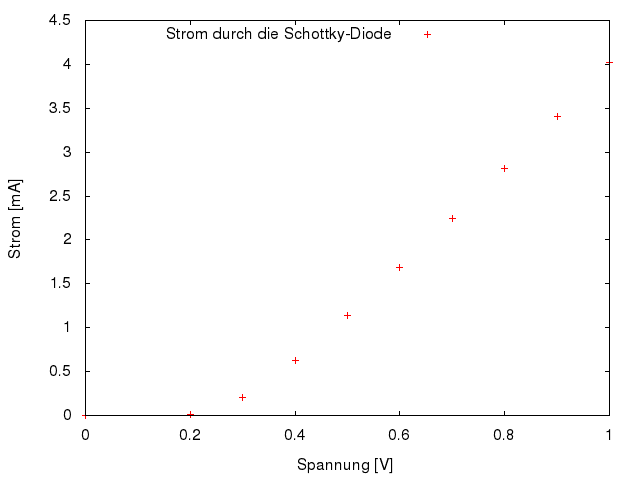
\includegraphics[width=\linewidth]{versuch2/versuch_2_2.png}
	\caption{Strom in Abhängigkeit der angelegten Spannung}
\end{figure}
Wie man leicht sieht, beginnt die Diode bei etwa 0.3 V nennenswert zu leiten.
%}}}

%{{{
\subsection{Kennlinie einer Leuchtdiode (rot)}
Im dritten Versuch der Reihe wurde die Schottky-Diode durch eine rote Leuchtdiode ausgetauscht. Deren Kennlinie ergab sich folgendermaßen:
\begin{figure}[H]
	\centering
	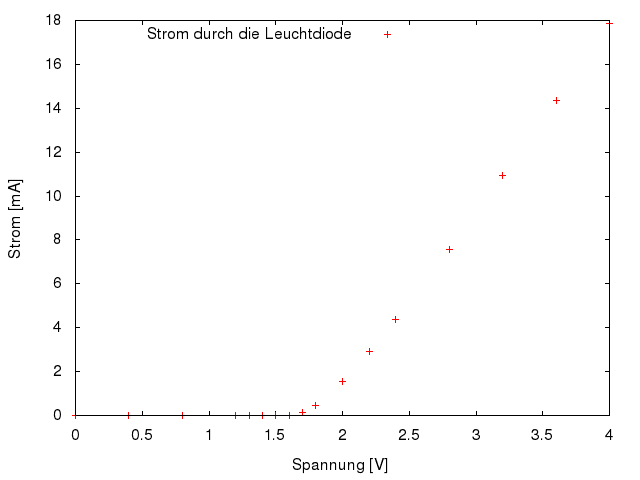
\includegraphics[width=\linewidth]{versuch2/versuch_2_3.png}
	\caption{Strom in Abhängigkeit der angelegten Spannung}
\end{figure}
Würde man statt der Roten ein blaue Leuchtdiode verwenden, würde sich der charakteristische Knick statt bei circa 1.6 V bei 2.9 V einstellen, da das die normale Schwellspannung bei blauen Leuchtdioden ist.

Würde man die LEDs ohne Vorwiderstand an einer Spannungsquelle betreiben, würden sie schlichtweg durchbrennen (siehe positiver Temperaturkoeffizient).
%}}}

%{{{
\subsection{Kennlinie der 1N4148 durch Simulation}
\begin{figure}[H]
	\centering
	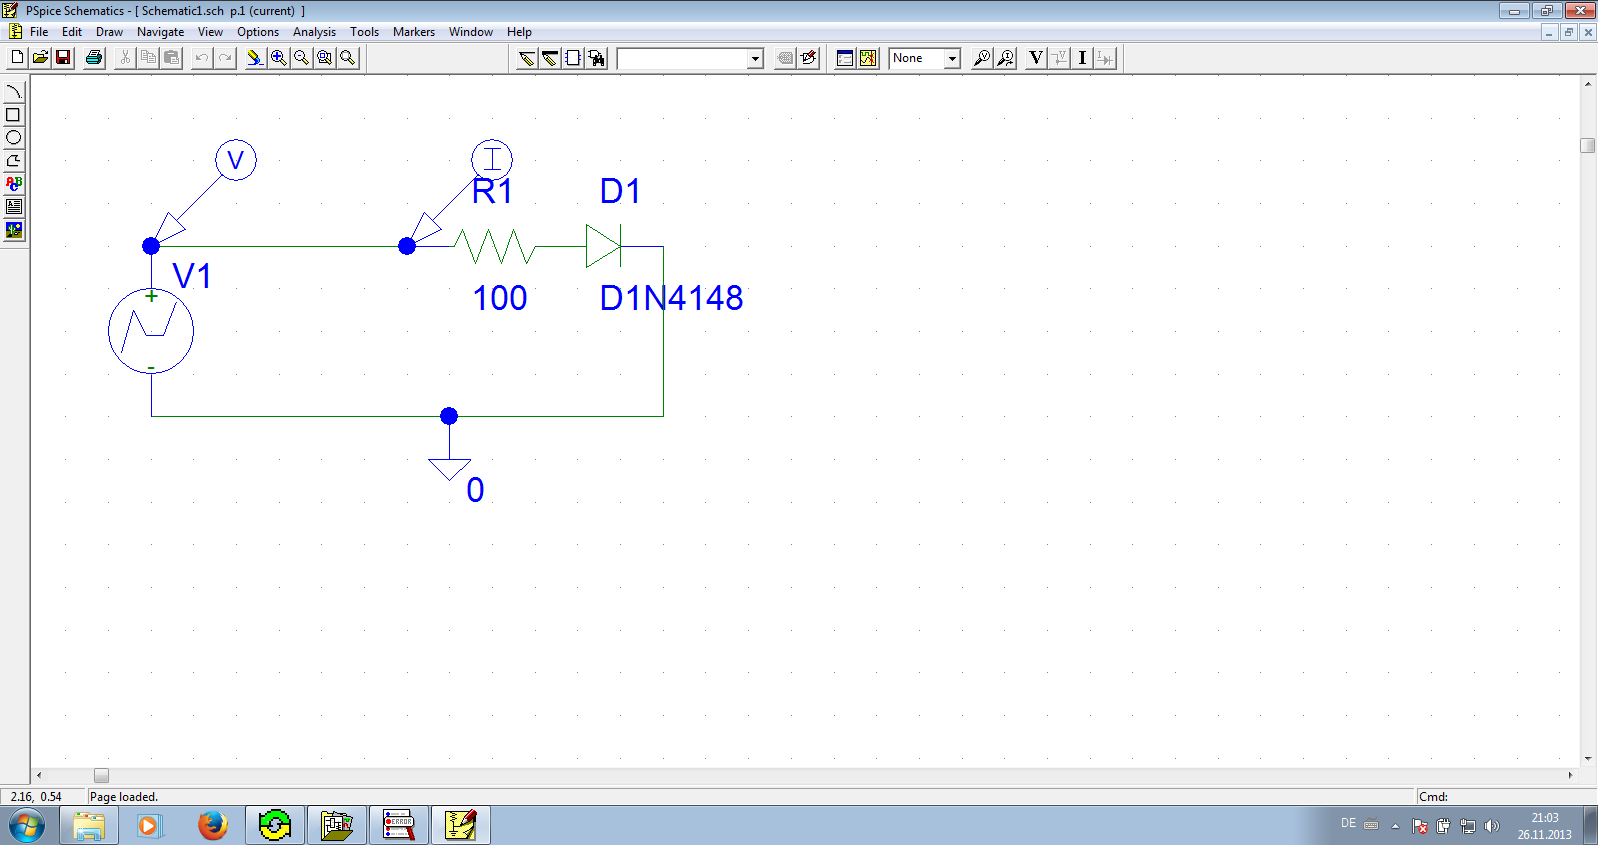
\includegraphics[width=\linewidth]{versuch2/spice/v2_4_1_schematic.png}
	\caption{Schaltplan für die Simulation mit Pspice}
\end{figure}
Einstellungen der Signalquelle: VPWL: DC = 0V; AC = 0V; T1 = 0s; V1 = 0V; T2 = 2s; V2 = 2V\\
\begin{figure}[H]
	\centering
	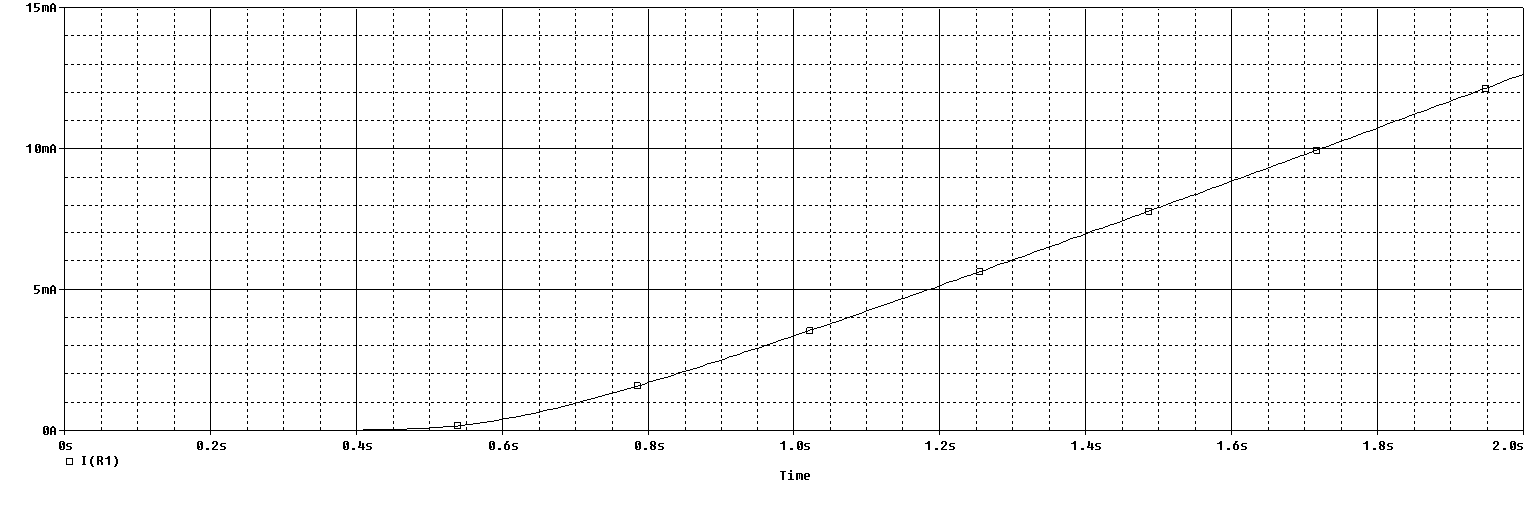
\includegraphics[width=\linewidth]{versuch2/spice/v2_4_1_simulation.png}
	\caption{Und die Simulationsergebnisse}
\end{figure}
Mit den geänderten Einstellungen: VPWL: DC = 0V; AC = 0V; T1 = 0s; V1 = -5V; T2 = 10s; V2 = +5V ergibt sich:
\begin{figure}[H]
	\centering
	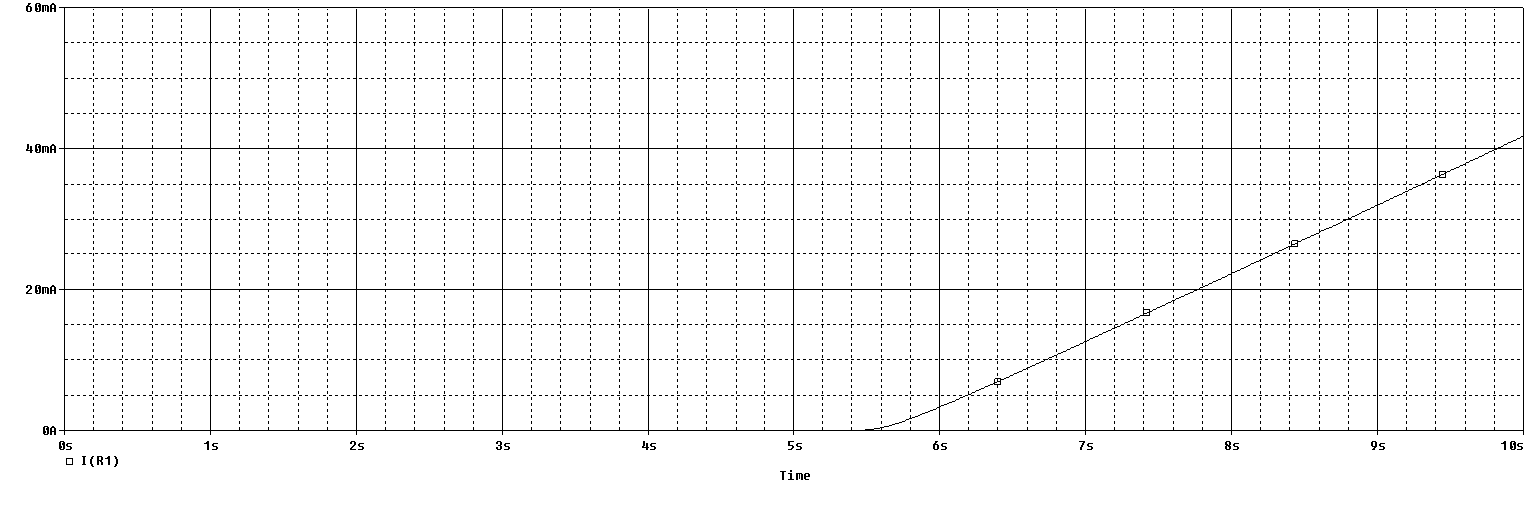
\includegraphics[width=\linewidth]{versuch2/spice/v2_4_2_simulation.png}
	\caption{Und die Simulationsergebnisse}
\end{figure}
In der Simulation beginnt die Diode bei etwa 0.25 V zu leiten. Die Simulation vernachlässigt die Erwärmung der Diode. Und eine perfekte Diode hat überhalb ihrer Schwellspannung das gleiche lineare Verhalten wie ein Ohm'scher Widerstand. Daher ist der Stromanstieg im Durchlassbereich linear.
%}}}

%{{{
\subsection{Halbwellengleichrichter}
\begin{figure}[H]
	\centering
	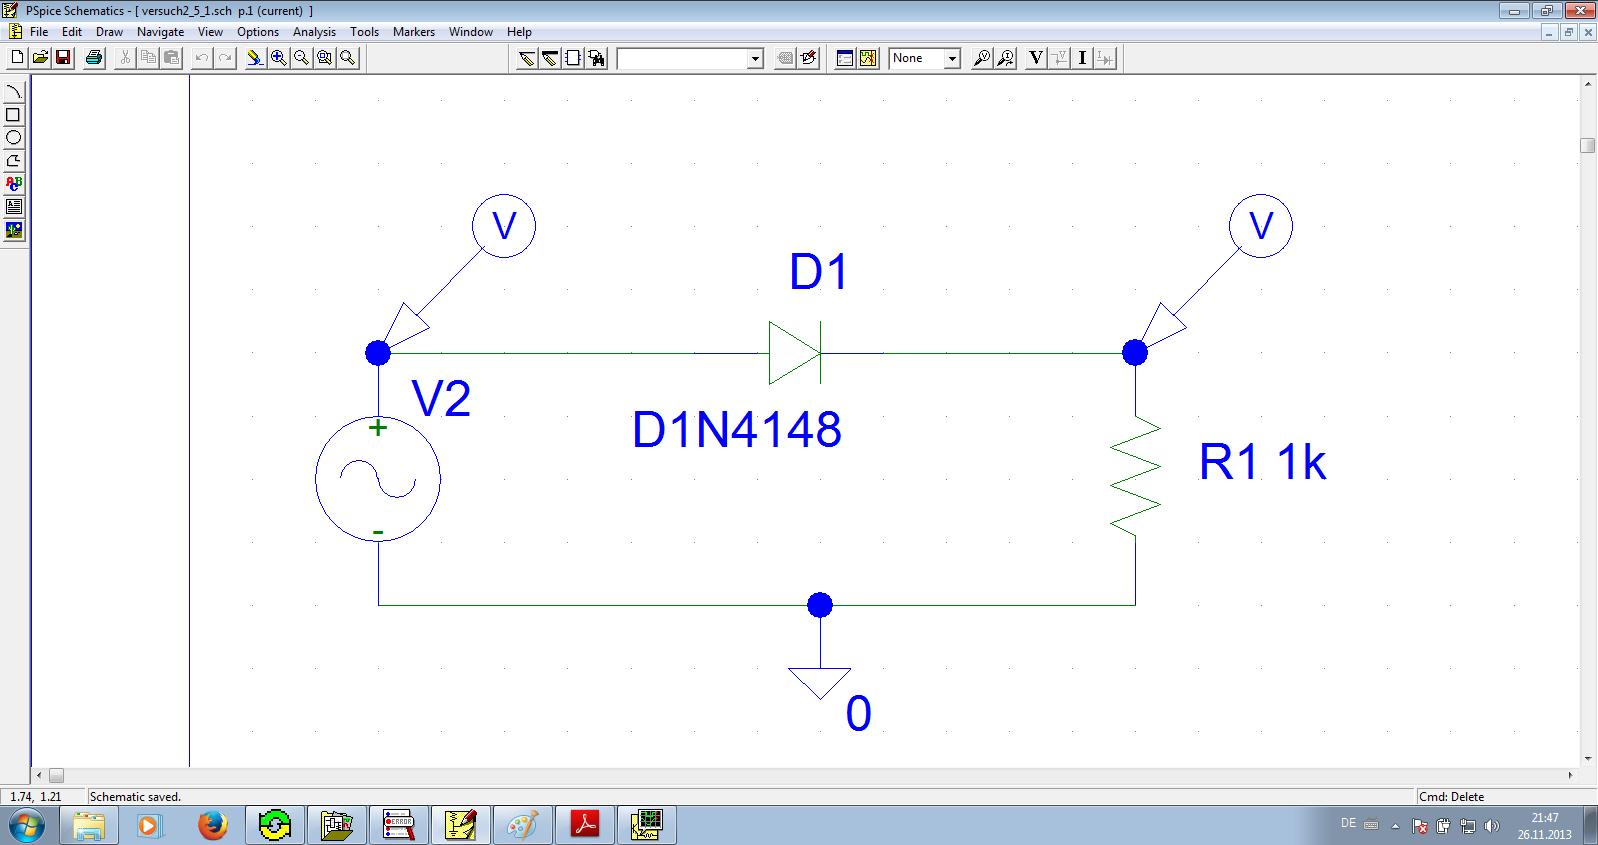
\includegraphics[width=\linewidth]{versuch2/spice/v2_5_1_schematic.png}
	\caption{Schaltplan für die Simulation mit Pspice}
\end{figure}
Einstellungen der Signalquelle: VSIN: DC = 0; AC = 0; VOFF = 0; VAMPL = 10V; FREQ = 50;
\begin{figure}[H]
	\centering
	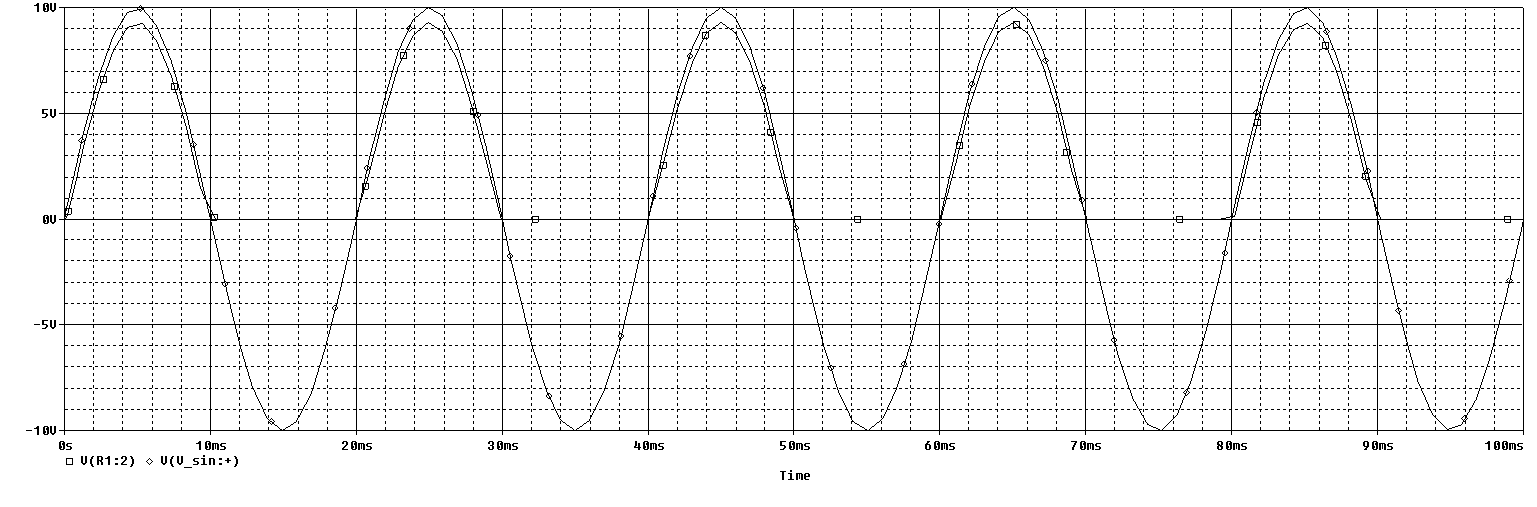
\includegraphics[width=\linewidth]{versuch2/spice/v2_5_1_simulation.png}
	\caption{Und die Simulationsergebnisse}
\end{figure}
Man sieht, dass die Spannung am Widerstand während der positiven Halbwelle rund 0.7 V kleiner ist als die der Spannungsquelle. Hier zeigt sich die Durchlassspannung der Diode.

Nun fügte ich einen Glättkondensator hinzu:
\begin{figure}[H]
	\centering
	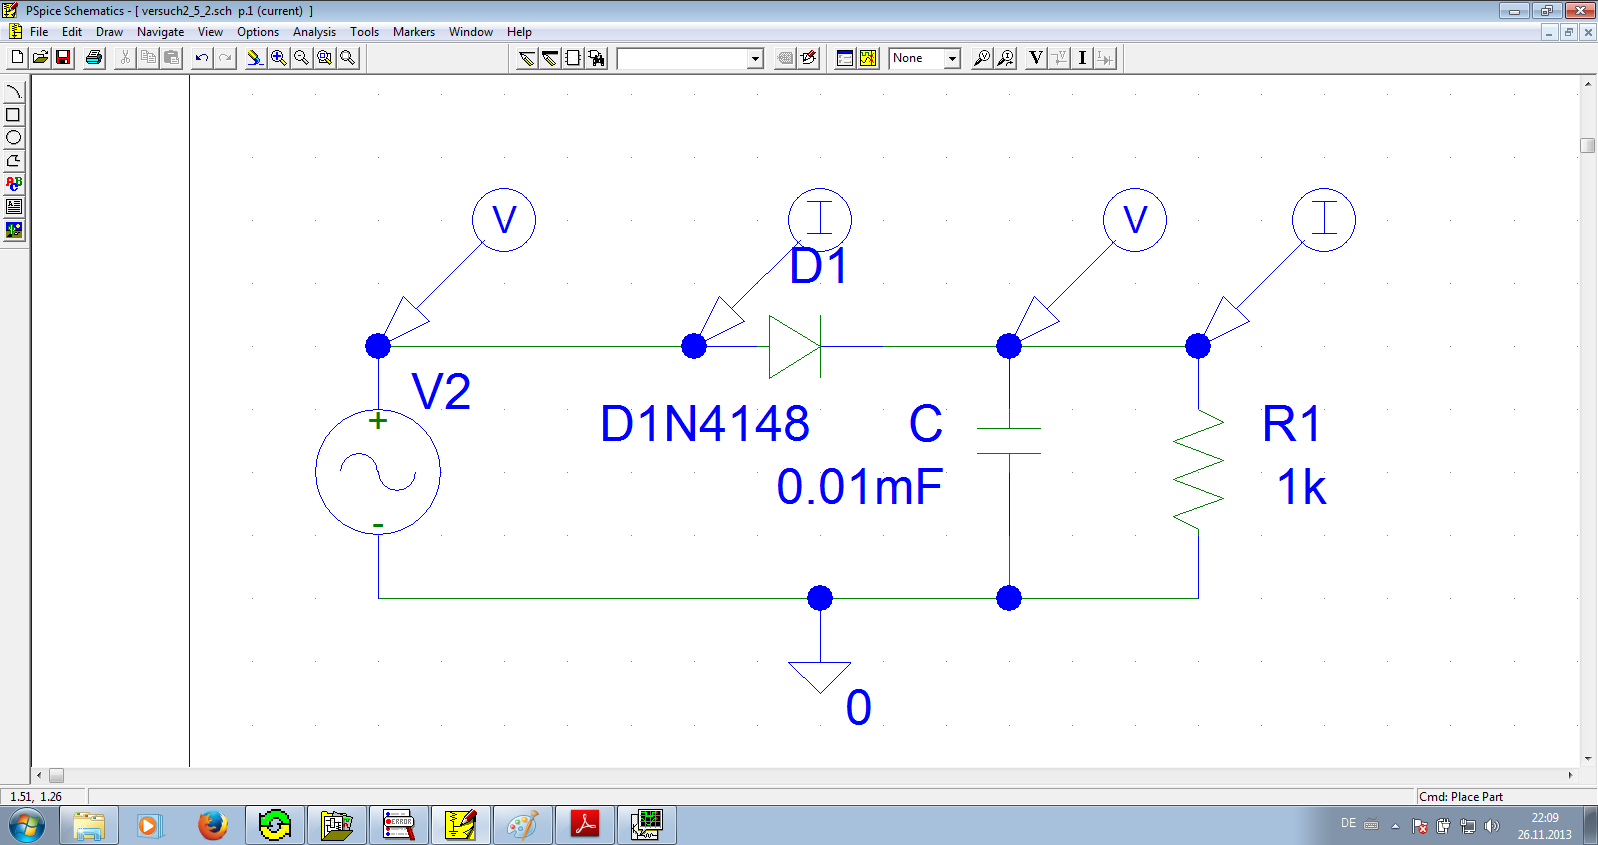
\includegraphics[width=\linewidth]{versuch2/spice/v2_5_2_schematic.png}
	\caption{Schaltplan für die Simulation mit Pspice}
\end{figure}
Sofern der Kondensator groß genug ist, würde ich einen mittleren Strom knapp kleiner als $ I=10V/1010\Omega = 0.0099010 A = 9.9010 mA $ erwarten, da nur die positive Halbwelle zur Verfügung steht.\\
Die Simulation hingegen zeigt:
\begin{figure}[H]
	\centering
	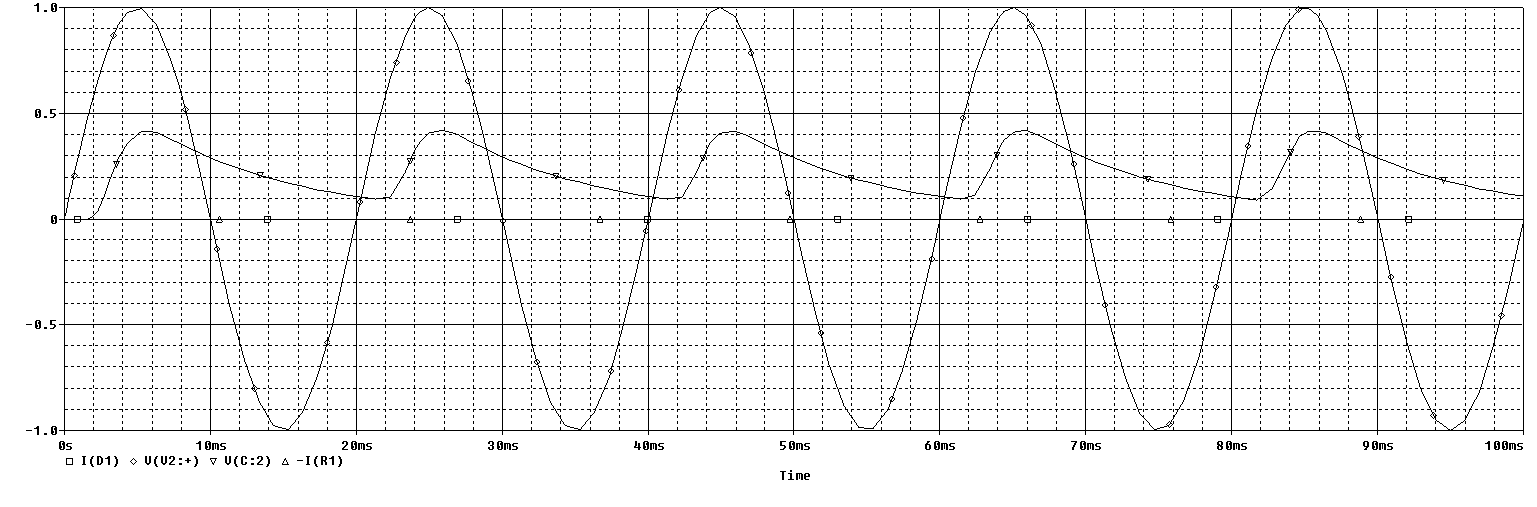
\includegraphics[width=\linewidth]{versuch2/spice/v2_5_2_simulation.png}
	\caption{Und die Simulationsergebnisse}
\end{figure}
Und noch einmal der Strom am Widerstand:
\begin{figure}[H]
	\centering
	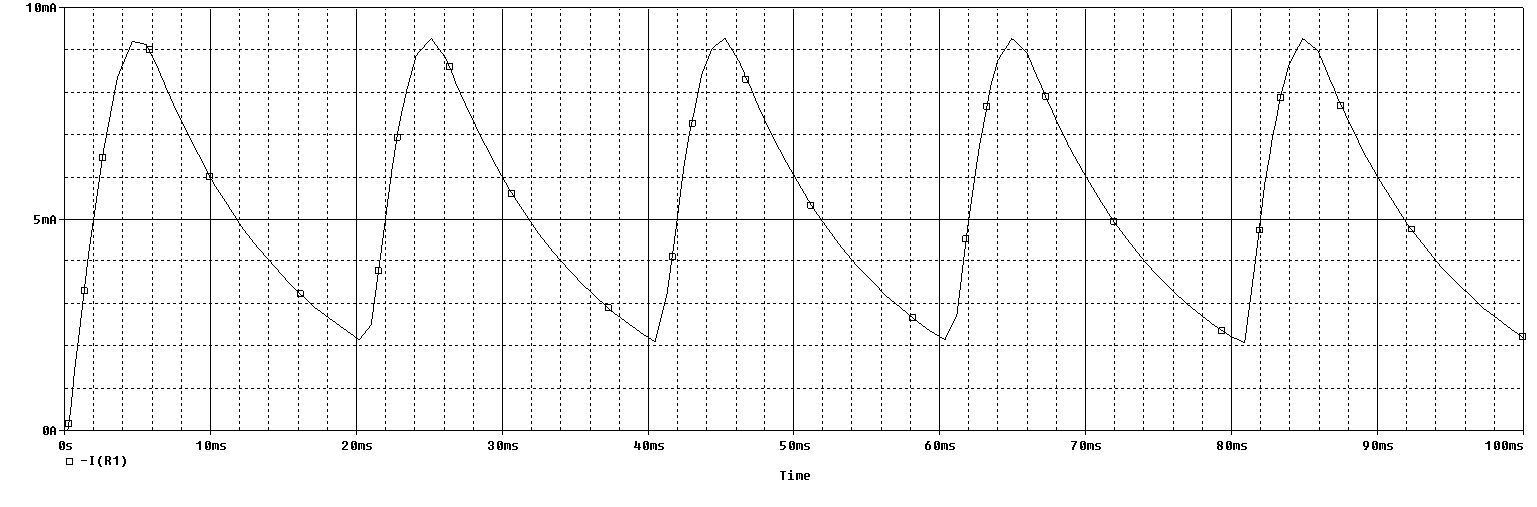
\includegraphics[width=\linewidth]{versuch2/spice/v2_5_2_strom_simulation.png}
	\caption{Und die Simulationsergebnisse}
\end{figure}
Man sieht, dass der Kondensator zu klein gewählt ist, da der Strom noch nicht ausreichend geglättet ist.\\
Wenn man nun die Kapazität auf 1 mF erhöht, ergibt sich folgende Simulation:
\begin{figure}[H]
	\centering
	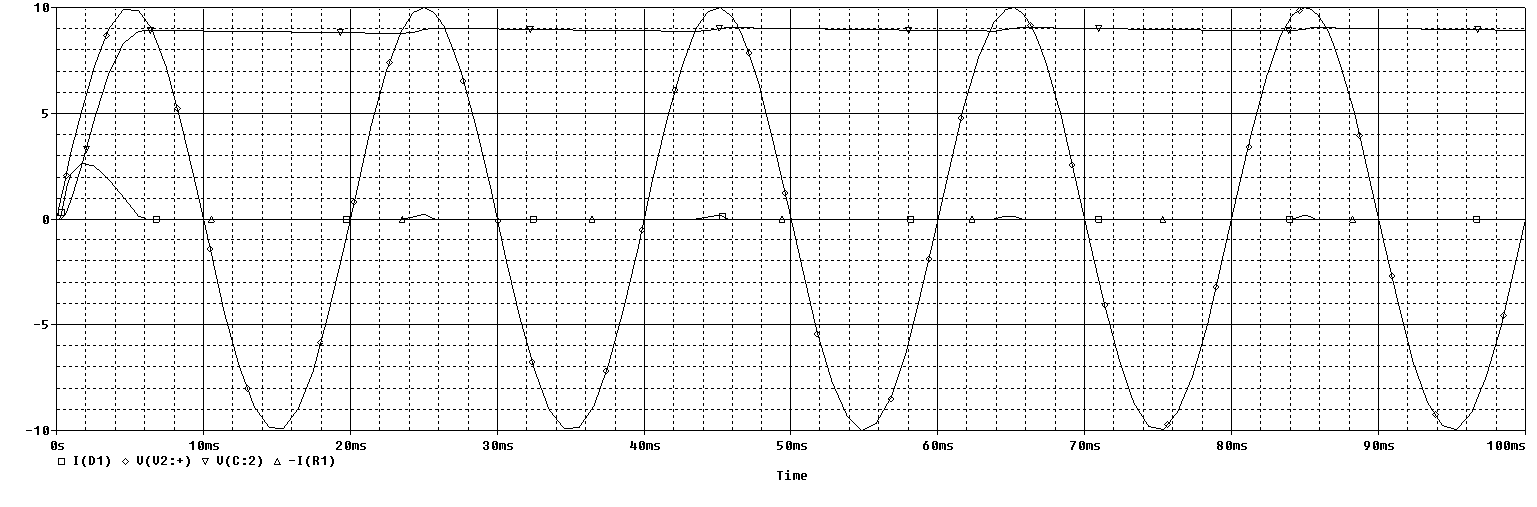
\includegraphics[width=\linewidth]{versuch2/spice/v2_5_3_simulation.png}
	\caption{Und die Simulationsergebnisse}
\end{figure}
Und noch einmal der Strom am Widerstand:
\begin{figure}[H]
	\centering
	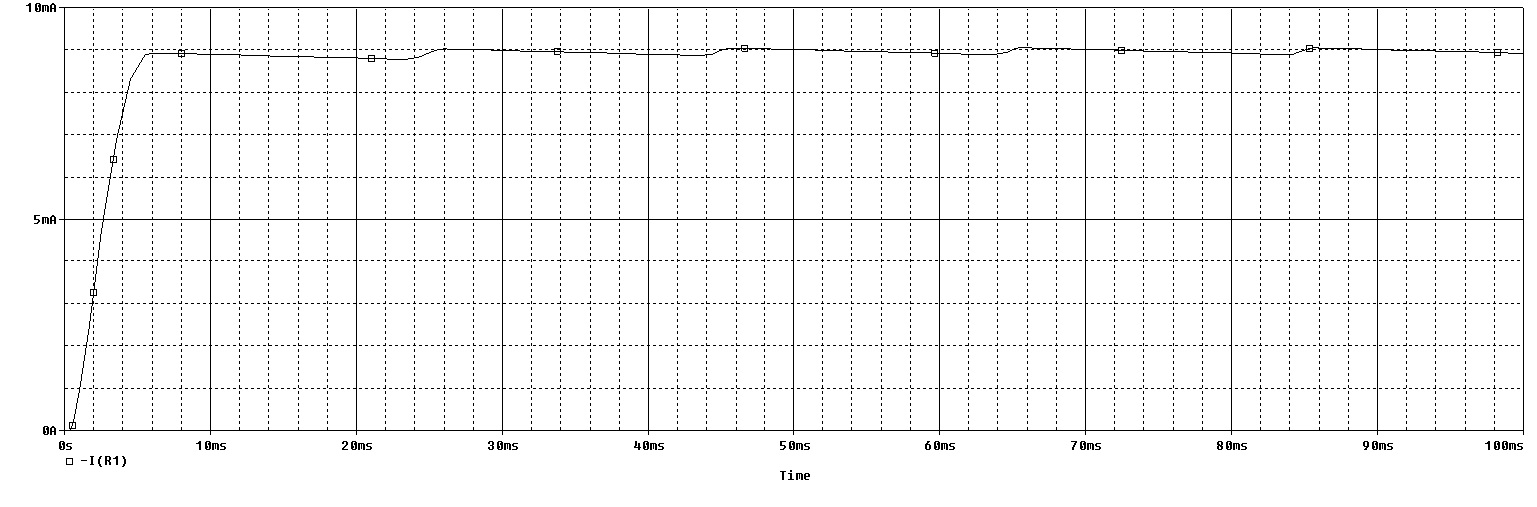
\includegraphics[width=\linewidth]{versuch2/spice/v2_5_3_strom_simulation.png}
	\caption{Und die Simulationsergebnisse}
\end{figure}
Wie man sieht, wird der Strom deutlich besser geglättet. Der Preis für diese Verbesserung ist jedoch der größere Preis und Platzbedarf des Kondensators, sowie der größere Strom beim Einschalten, bis der Kondensator geladen ist. Bei Leistungsnetzteilen kann dieser, sofern keine entsprechende Schutzbeschaltung vorhanden ist, so groß werden, dass die Haussicherung anspricht. Falls die Sicherung nicht anspricht, stellt der große Strom jedoch auch für das Netzteil selbst eine große Belastung dar, da die Bauteile meist für die Dauerbelastung ausgelegt sind, die deutlich geringer ist. So kann es bei zu schwach dimensionierten Bauteilen insbesondere bei der Gleichrichterdiode zum Entweichen des magischen Rauches kommen.

Als nächstes habe ich die Amplitude der Spannungsquelle auf 1 V verringert.
\begin{figure}[H]
	\centering
	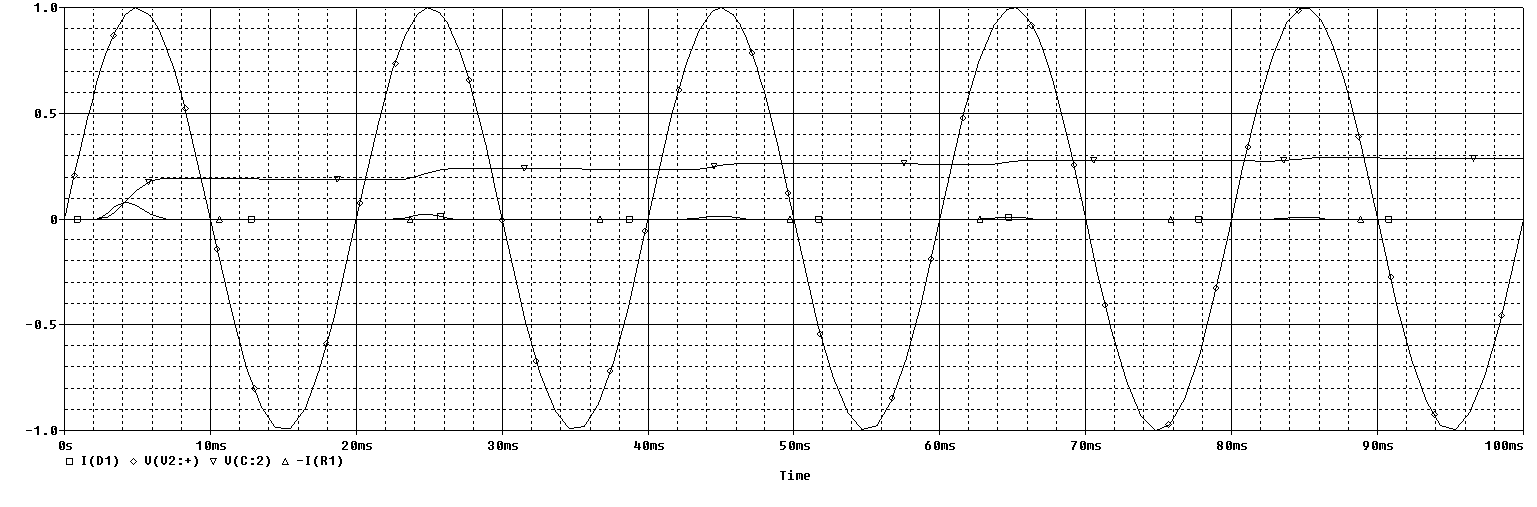
\includegraphics[width=\linewidth]{versuch2/spice/v2_5_4_simulation.png}
	\caption{Und die Simulationsergebnisse}
\end{figure}
Wie man sieht, ist der Kondensator nach den ersten Schwingungen noch nicht voll aufgeladen, daher habe ich die Simulationszeit erhöht:
\begin{figure}[H]
	\centering
	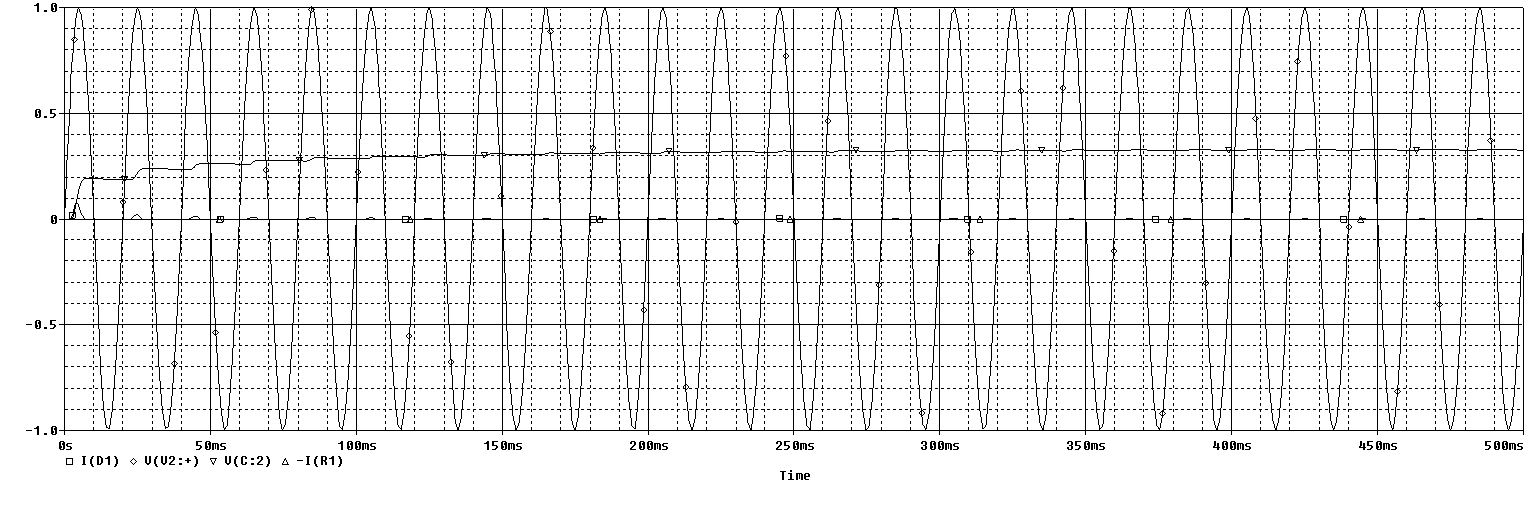
\includegraphics[width=\linewidth]{versuch2/spice/v2_5_4_2_simulation.png}
	\caption{Und die Simulationsergebnisse}
\end{figure}
Wie man sieht, nähert sich die Spannung an 0,4 V an, der Strom durch den Widerstand nähert sich an 0,31 A. Damit ergäbe sich ein Spannungsabfall von 0,6 V. Entfernt man den Widerstand, so erkennt man, dass dieser Wert auch ohne Widerstand stimmt (und mir fiel keine bessere Methode ein, den Widerstand rauszurechnen, ohne wenigstens die Spannung zu ändern).\\
Ersetzt man die Diode durch die Schottky-Diode MBD101, so steigt die Ausgangsspannung des Gleichrichters auf 5,5 V an, der Spannungsabfall beträgt somit nur noch 4,5 V. Entfernt man den Widerstand, so erhält man den reinen Spannungsabfall an der Diode mit 3.9 V.

Nun habe ich die Schaltung real aufgebaut und das Oszilloskop nach Vorgabe angeschlossen. Leider habe ich dabei die Bedienung der Cursorfunktion nicht auf Photos dokumentiert.
Zur Bestimmung der Brummspannung benutzte ich folgende Einstellung:
\begin{figure}[H]
	\centering
	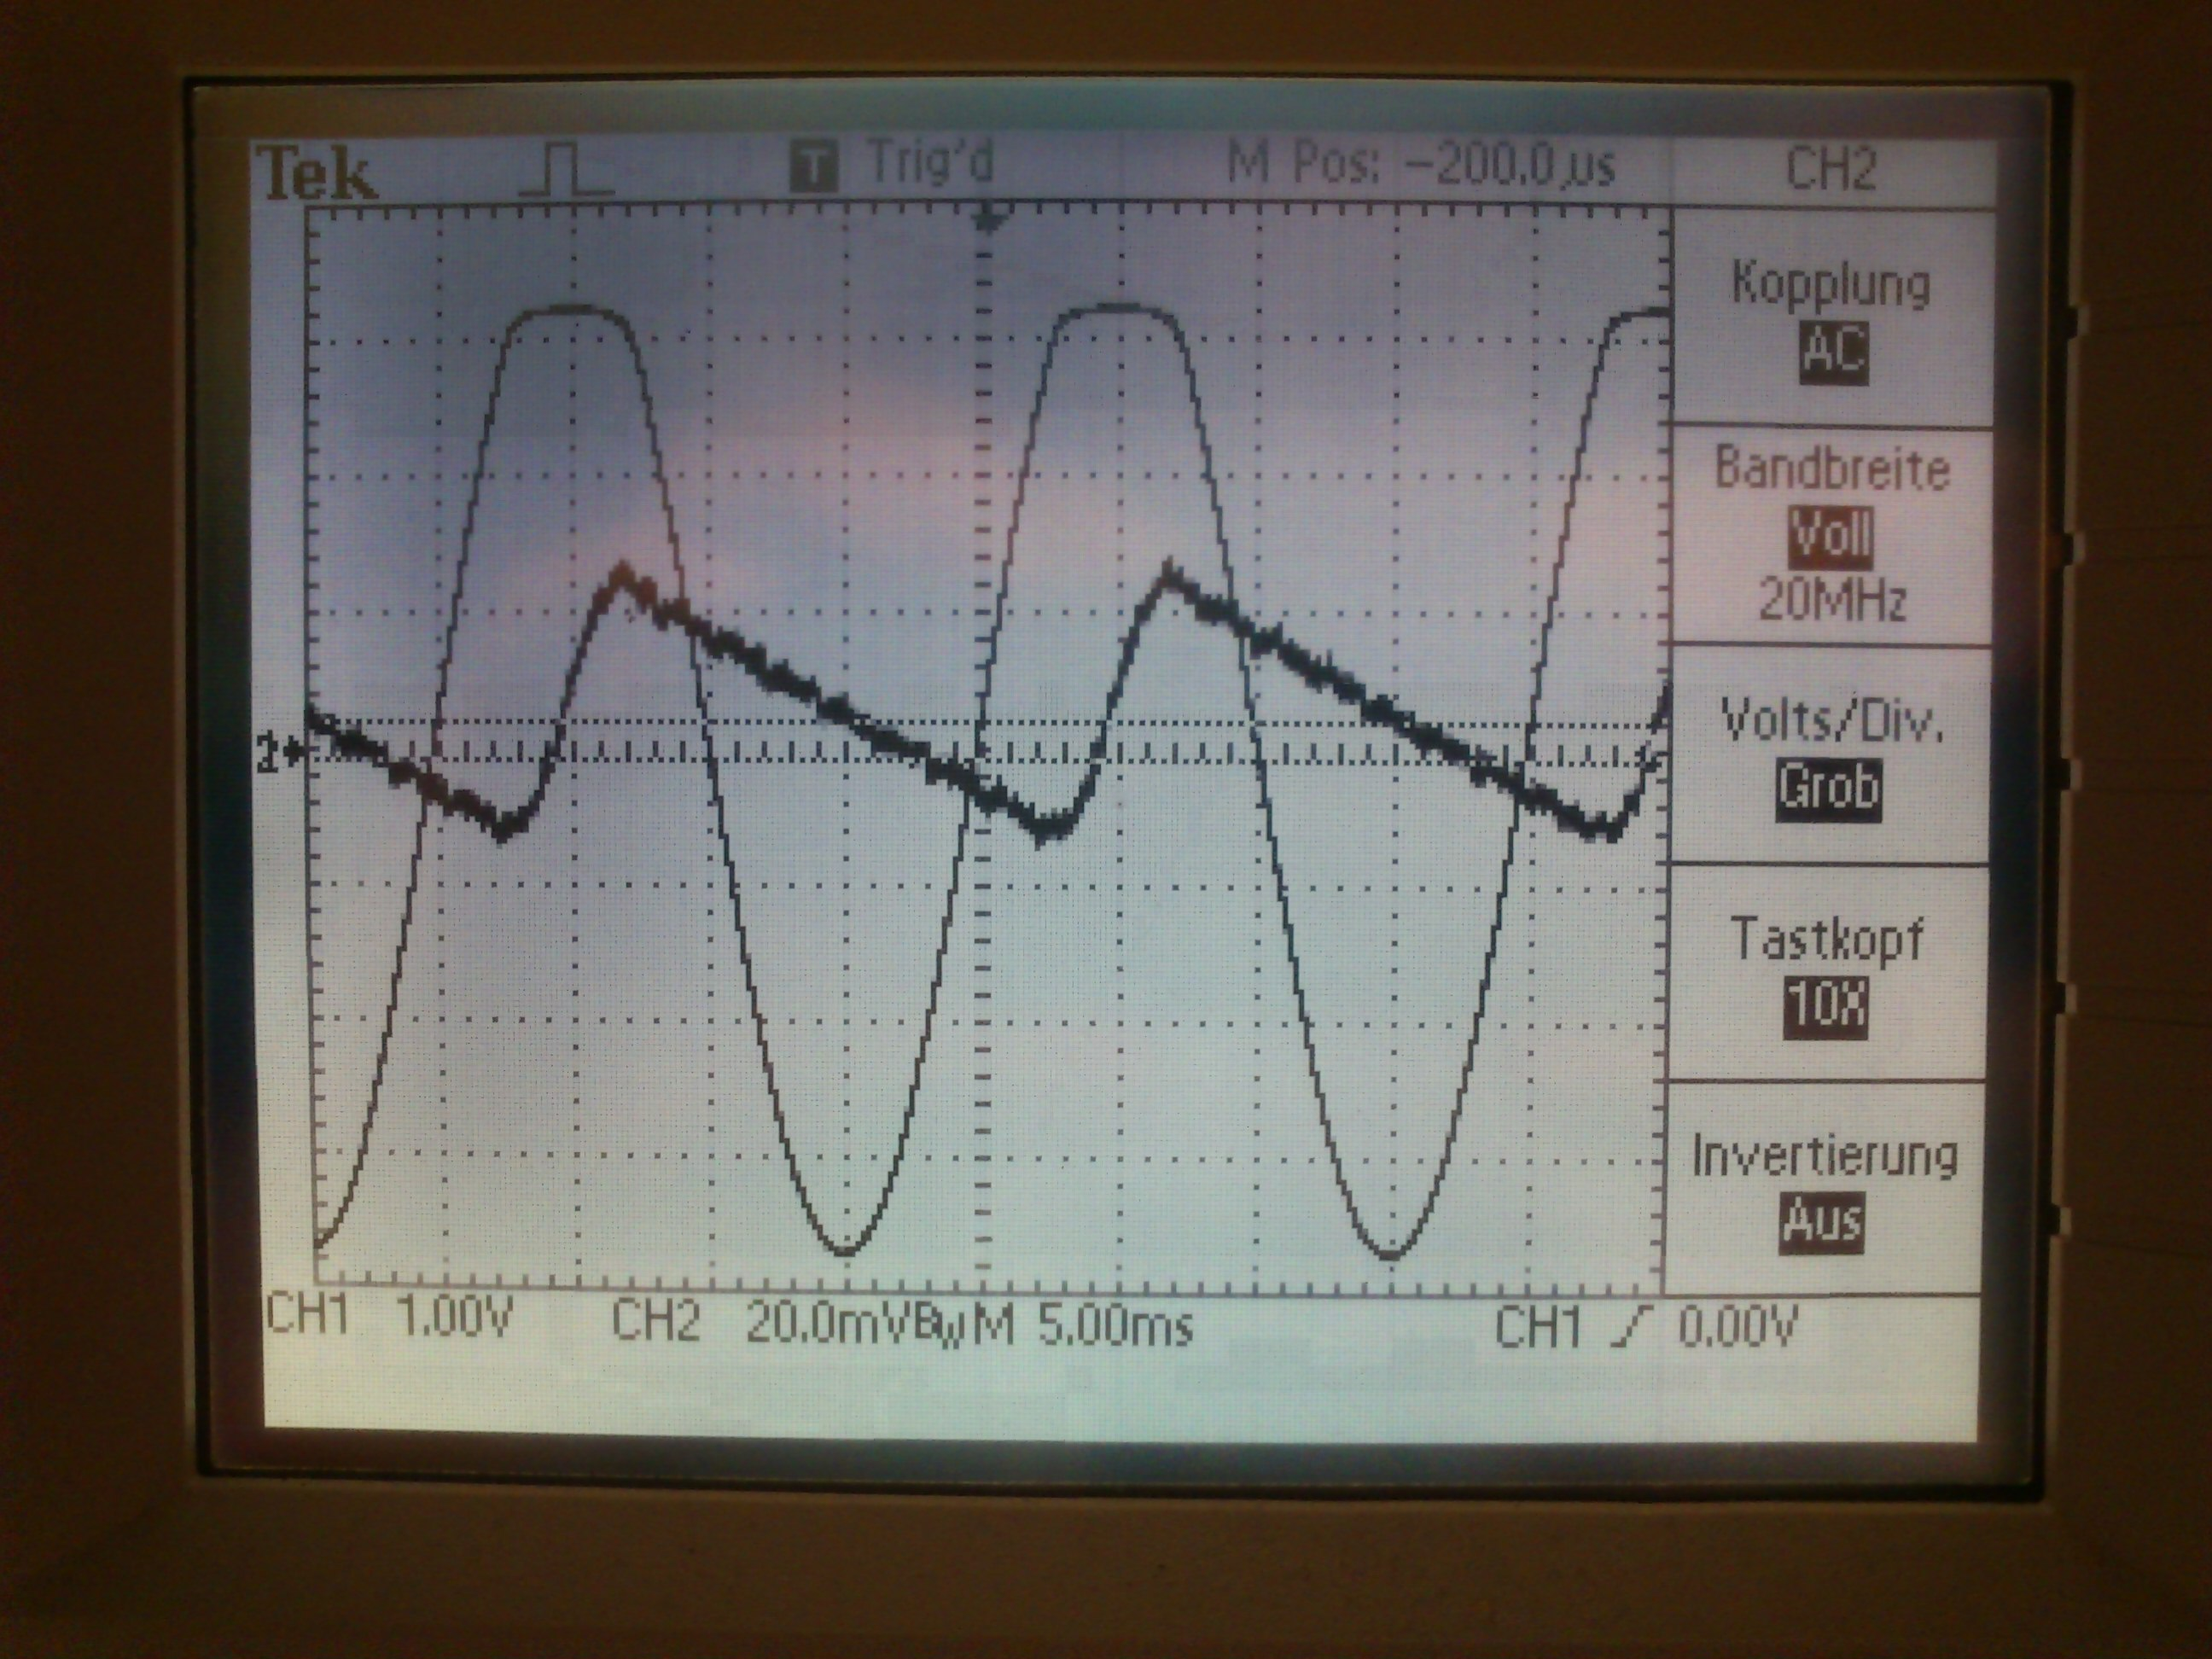
\includegraphics[width=\linewidth]{versuch2/oszi/DSC_0222.JPG}
	\caption{Messung der Brummspannung}
\end{figure}
Man erkennt leicht, dass die Brummspannung bei 40 mV liegt.\\
Die Gleichspannung ergibt sich zu 1.3 V, wie man am nächsten Bild ablesen kann:
\begin{figure}[H]
	\centering
	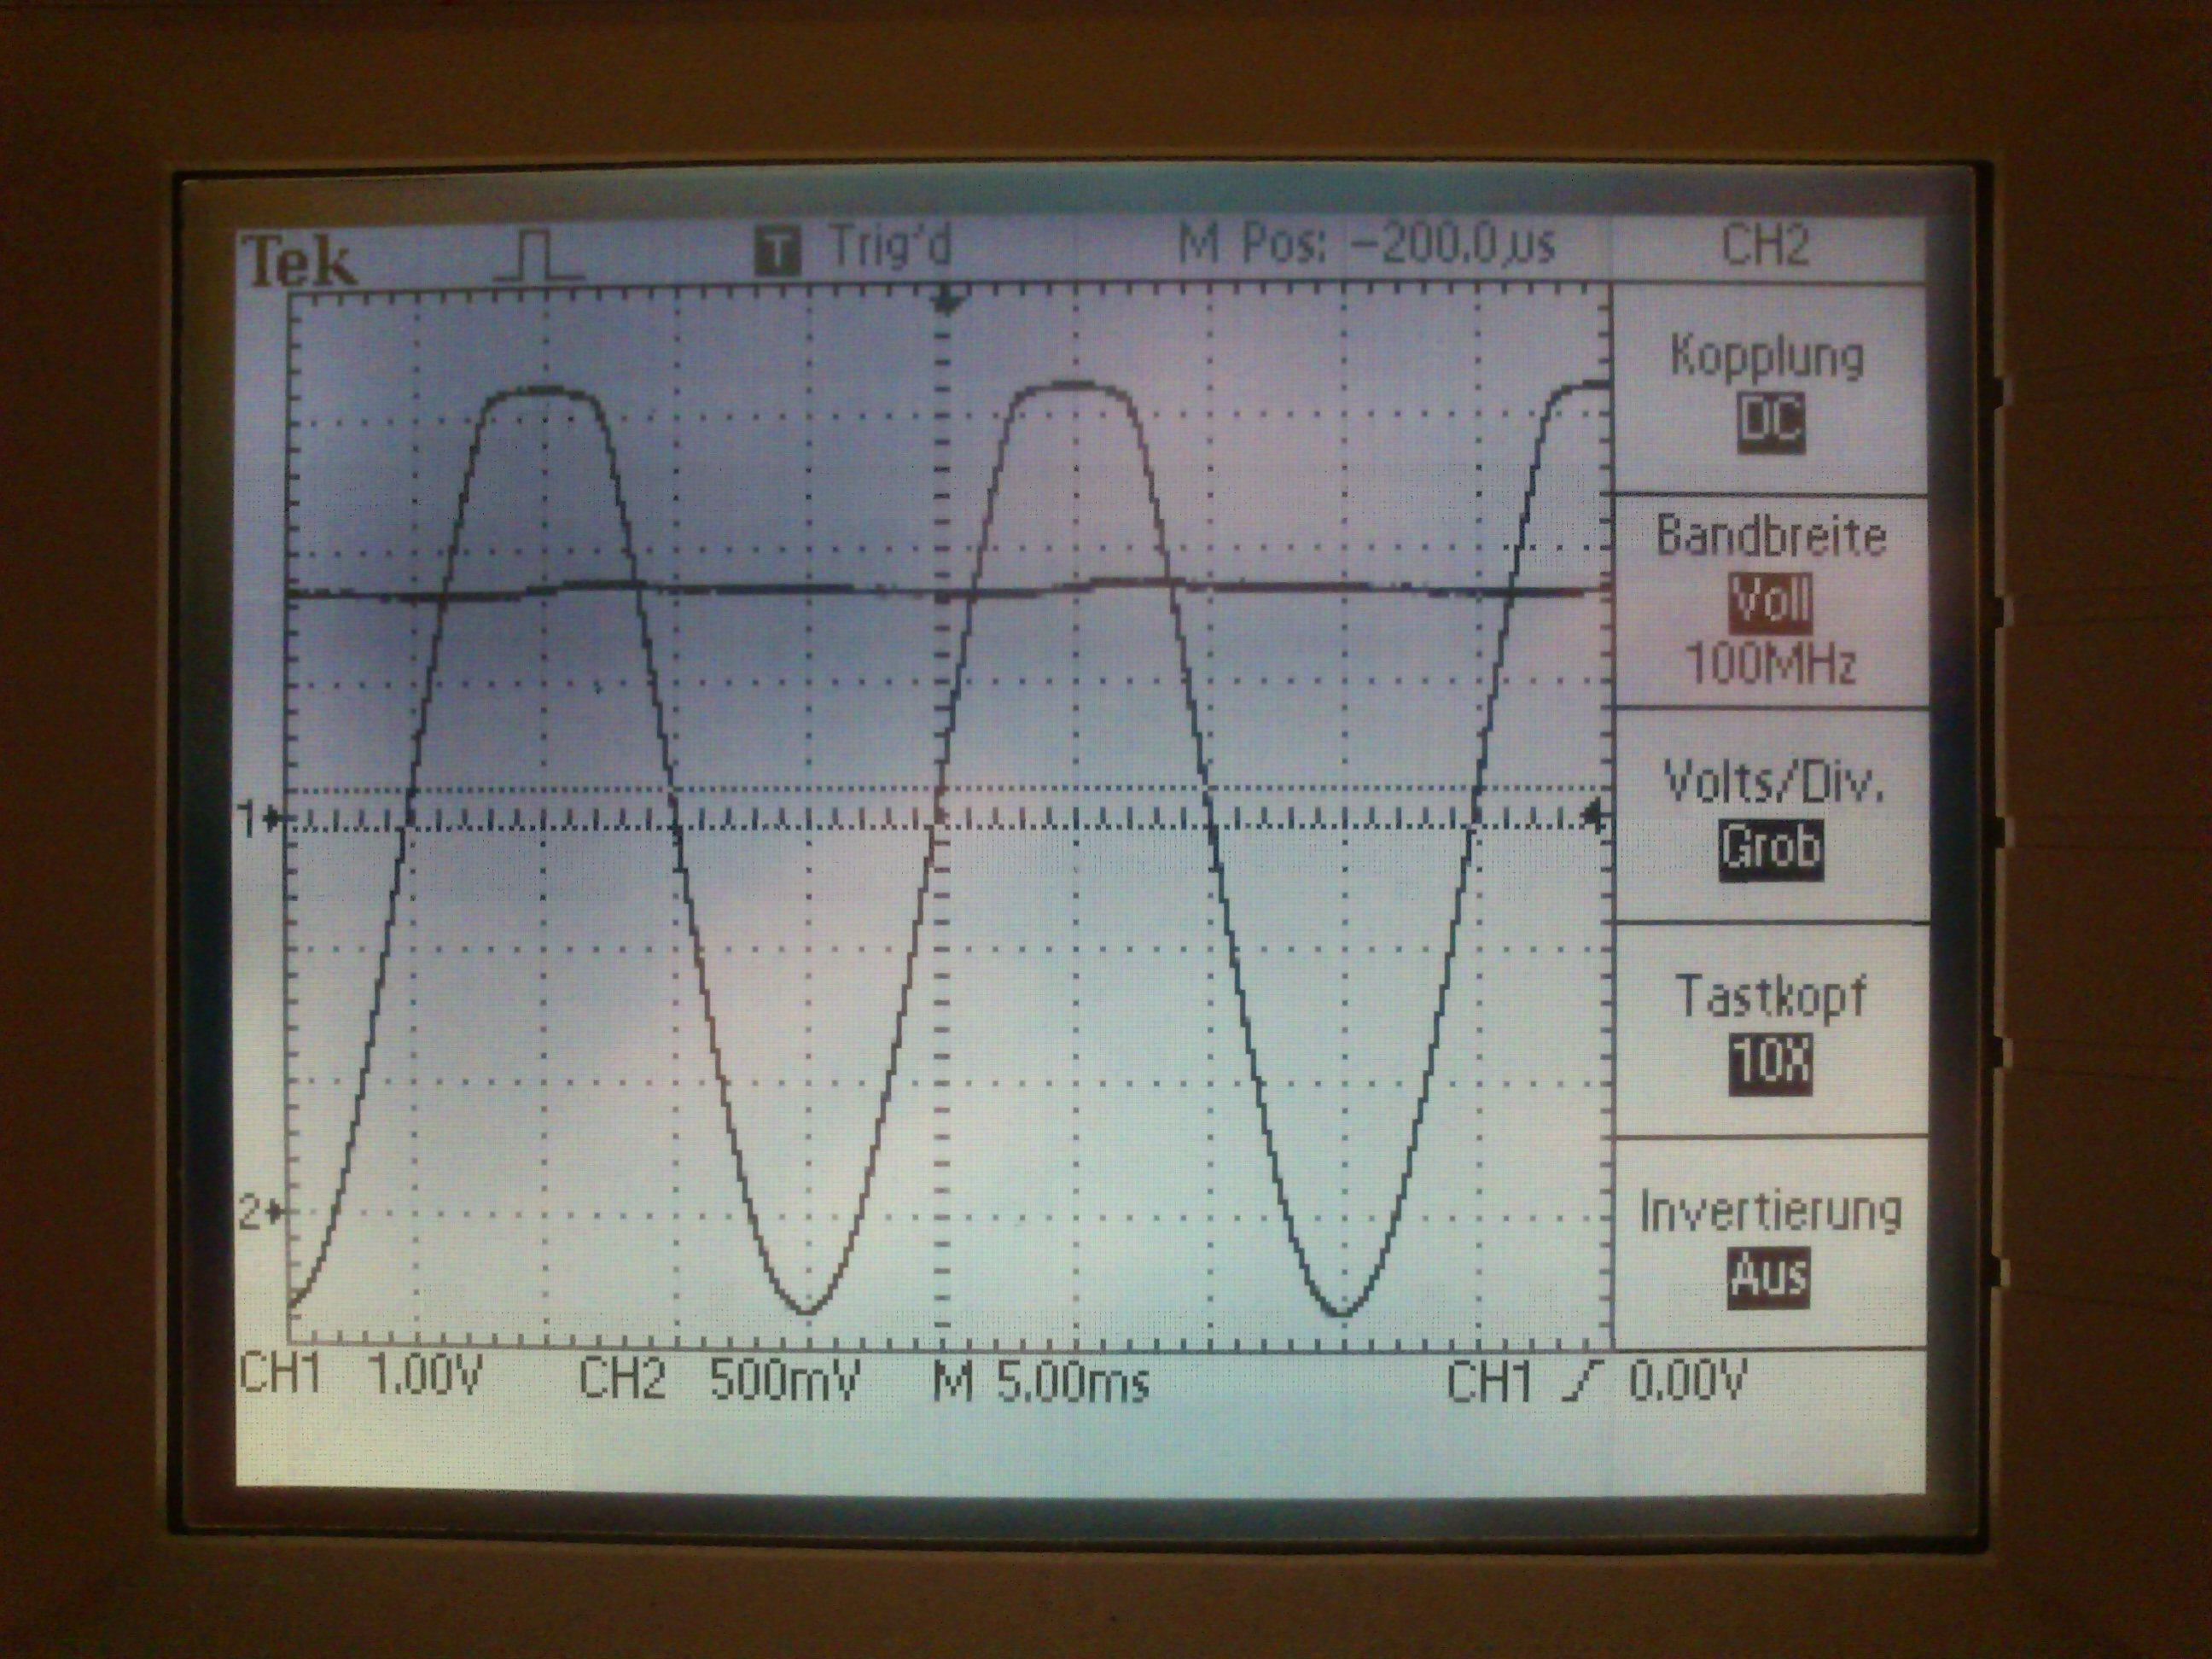
\includegraphics[width=\linewidth]{versuch2/oszi/DSC_0225.JPG}
	\caption{Messung der Gleichspannung}
\end{figure}
Somit beträgt der Spannungsverlust circa 0.7 V.
%}}}

%{{{
\subsection{Brückengleichrichter}
Ich habe folgende Schaltung im Pspice eingegeben:
\begin{figure}[H]
	\centering
	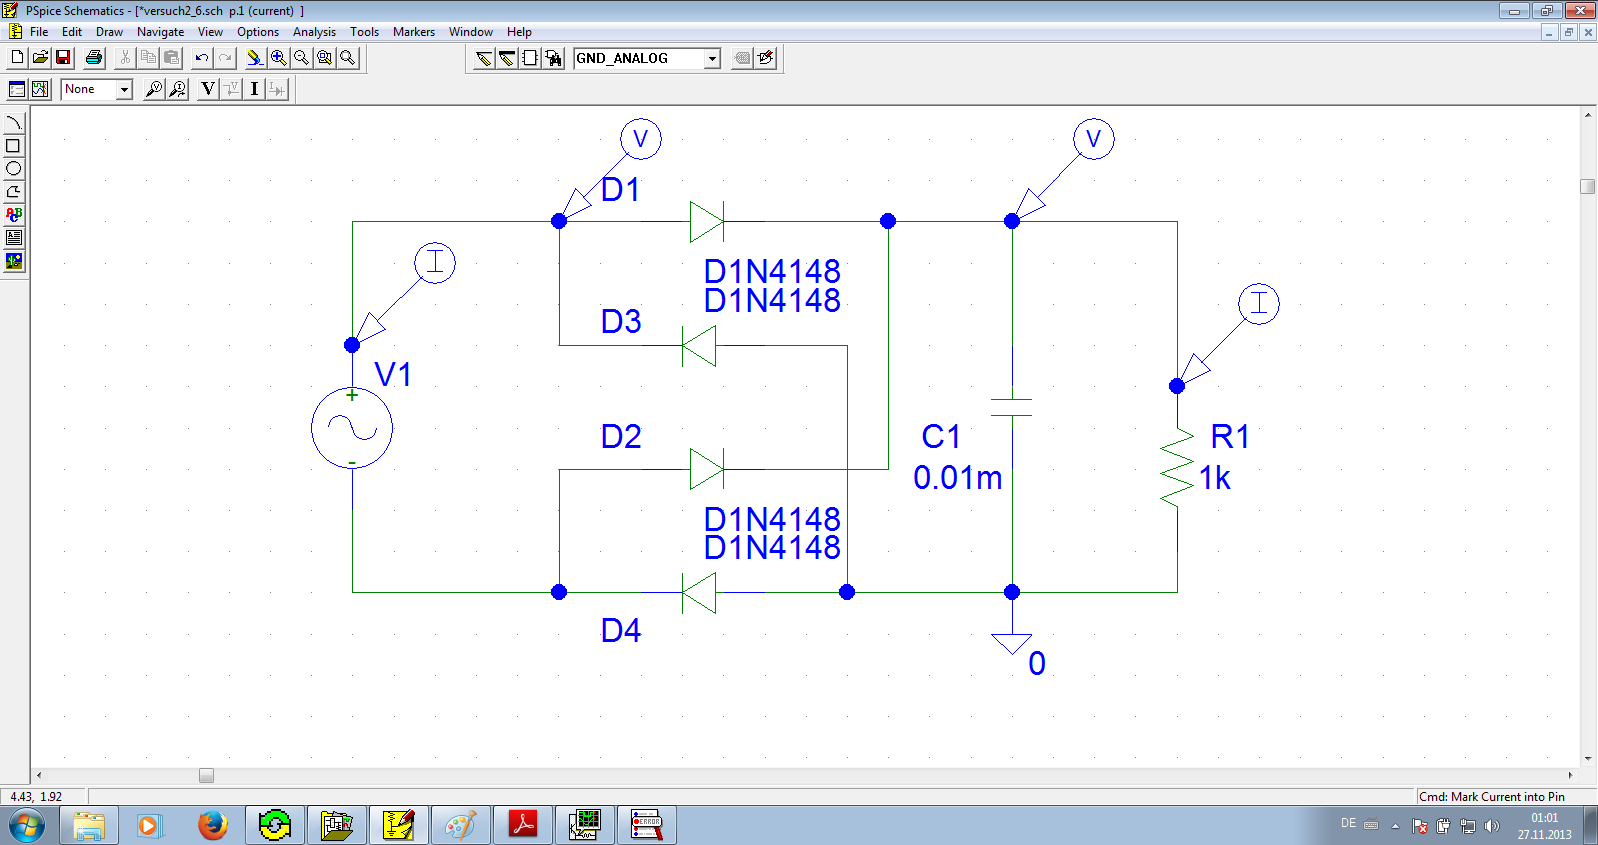
\includegraphics[width=\linewidth]{versuch2/spice/v2_6_1_schematic.png}
	\caption{Schaltplan für die Simulation mit Pspice}
\end{figure}
Das ergab simuliert:
\begin{figure}[H]
	\centering
	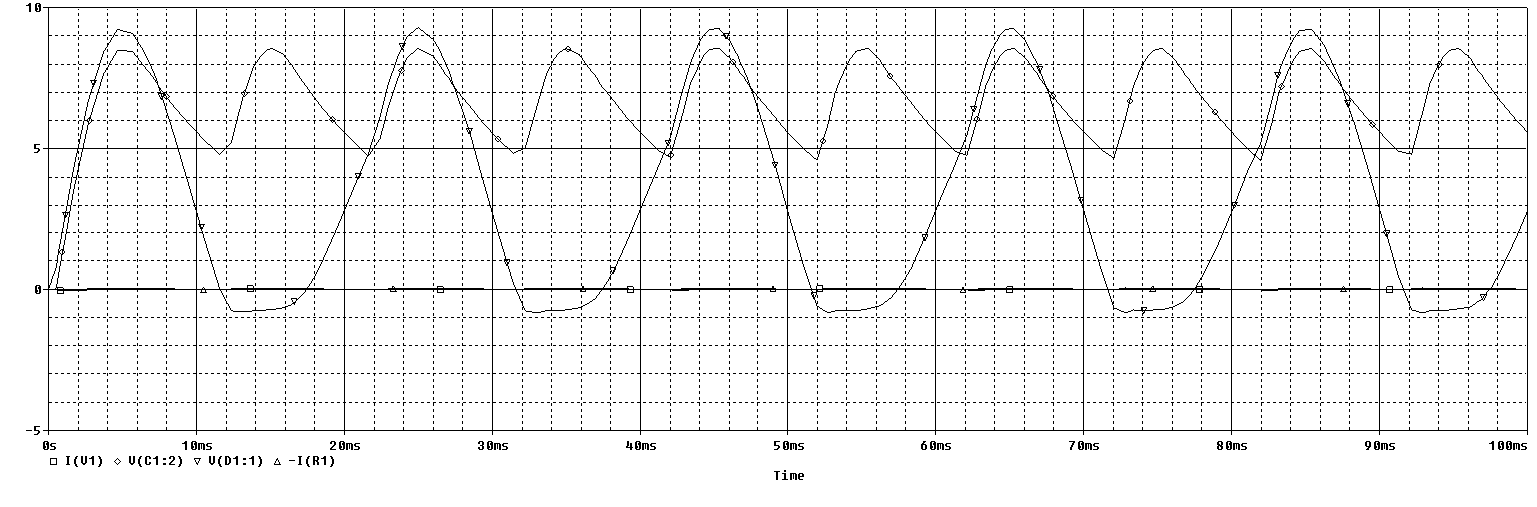
\includegraphics[width=\linewidth]{versuch2/spice/v2_6_1_simulation.png}
	\caption{Und die Simulationsergebnisse}
\end{figure}
Und noch einmal der Strom:
\begin{figure}[H]
	\centering
	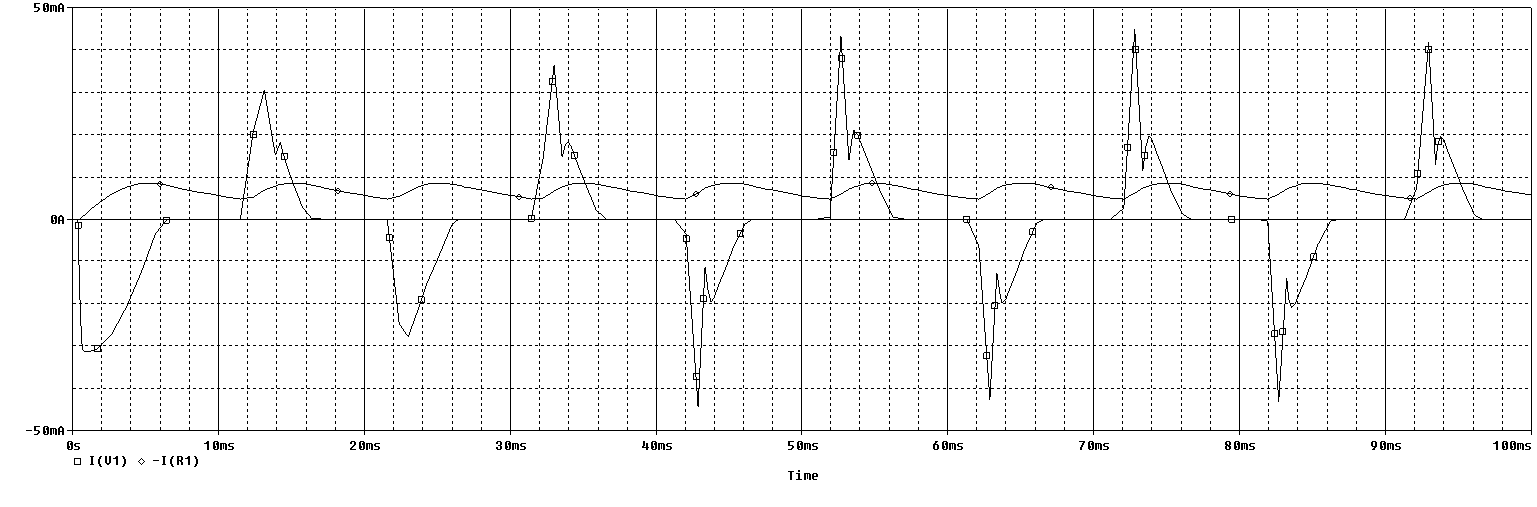
\includegraphics[width=\linewidth]{versuch2/spice/v2_6_1_strom_simulation.png}
	\caption{Und die Simulationsergebnisse}
\end{figure}
Da durch die Brückenschaltung beide Halbwellen genutzt werden können, muss der Kondensator den Strom nur noch halb so lange aufrecht erhalten. Somit kann er kleiner ausfallen, oder, sofern er gleich groß bleibt, wird der Strom glatter.
Wenn man die Kondensator auf 1 mF erhöht ist der Strom nahezu vollkommen gleichgerichtet:
\begin{figure}[H]
	\centering
	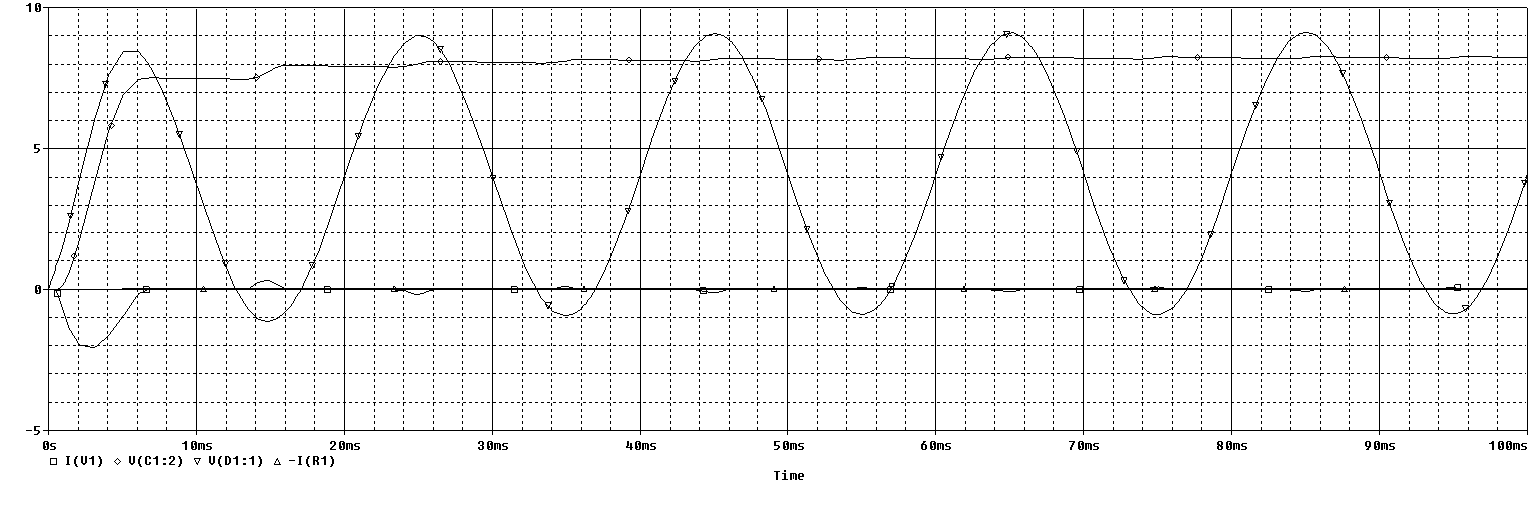
\includegraphics[width=\linewidth]{versuch2/spice/v2_6_2_simulation.png}
	\caption{Und die Simulationsergebnisse}
\end{figure}
Und noch einmal der Strom:
\begin{figure}[H]
	\centering
	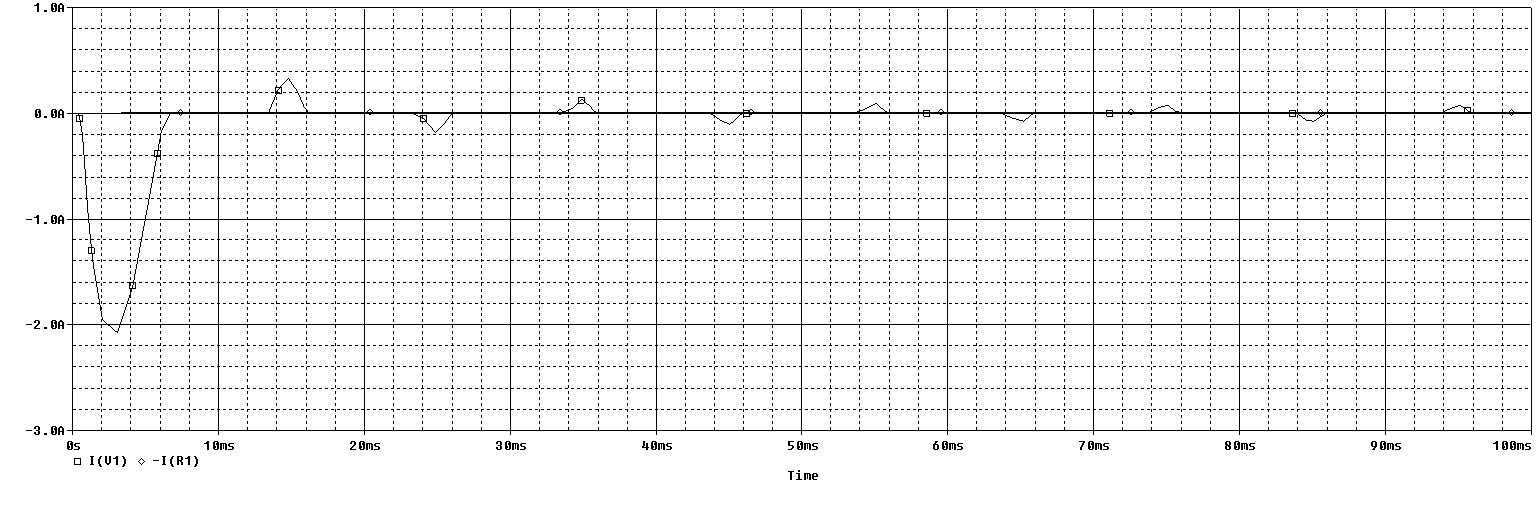
\includegraphics[width=\linewidth]{versuch2/spice/v2_6_2_strom_simulation.png}
	\caption{Und die Simulationsergebnisse}
\end{figure}
Die Vor- und Nachteile des größeren Kondensators sind die Gleichen wie beim Halbwellengleichrichter.\\
Die Dioden gehen beim Vollwellengleichrichter immer paarweise kaputt, weil immer 2 Dioden gleichzeitig leiten und somit immer 2 Dioden den gleichen Strom abbekommen.\\
Wenn man eine der Dioden umdreht, dann entsteht ein glatter Kurzschluss, der Strom würde nur durch den Widerstand der Dioden begrenzt. \textrightarrow viel magischer Rauch würde entweichen.

Als nächstes wurde folgende Schaltung simuliert:
\begin{figure}[H]
	\centering
	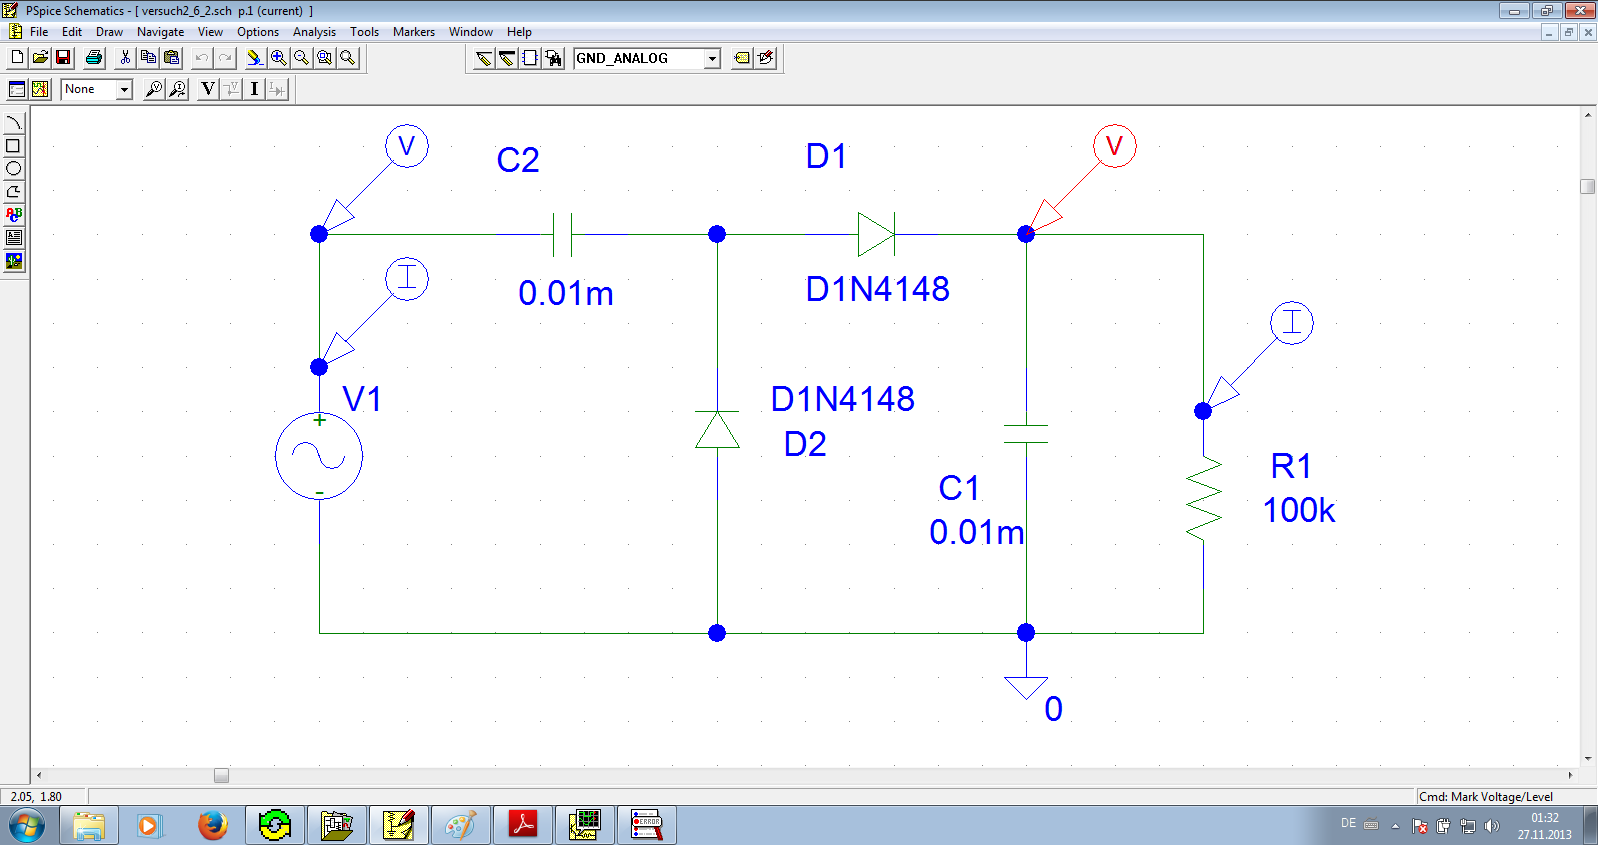
\includegraphics[width=\linewidth]{versuch2/spice/v2_6_3_schematic.png}
	\caption{Schaltplan für die Simulation mit Pspice}
\end{figure}
Das ergab simuliert:
\begin{figure}[H]
	\centering
	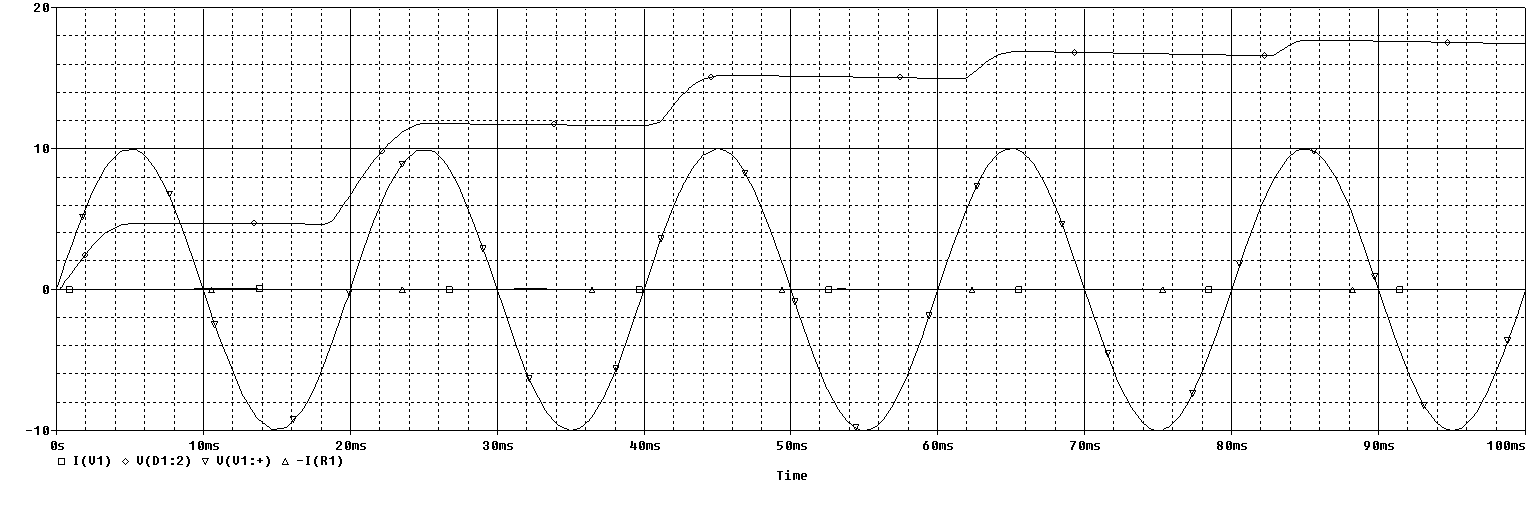
\includegraphics[width=\linewidth]{versuch2/spice/v2_6_3_simulation.png}
	\caption{Und die Simulationsergebnisse}
\end{figure}
Diese Simulation verwundert auf den ersten Blick, jedoch ist auch hier schnell eine Erklärung gefunden: Das System schwingt und erzeugt somit eine größere Spannung (wenn auch bei geringerer Stromstärke).
%}}}

%{{{
\subsection{Speicherzeit einer Diode}
Eine Diode wurde am Oszilloskop ausgemessen.\\
Die Speicherzeit lässt sich an folgendem Bild zu erkennen ist, beträgt die Speicherzeit 5µS.
\begin{figure}[H]
	\centering
	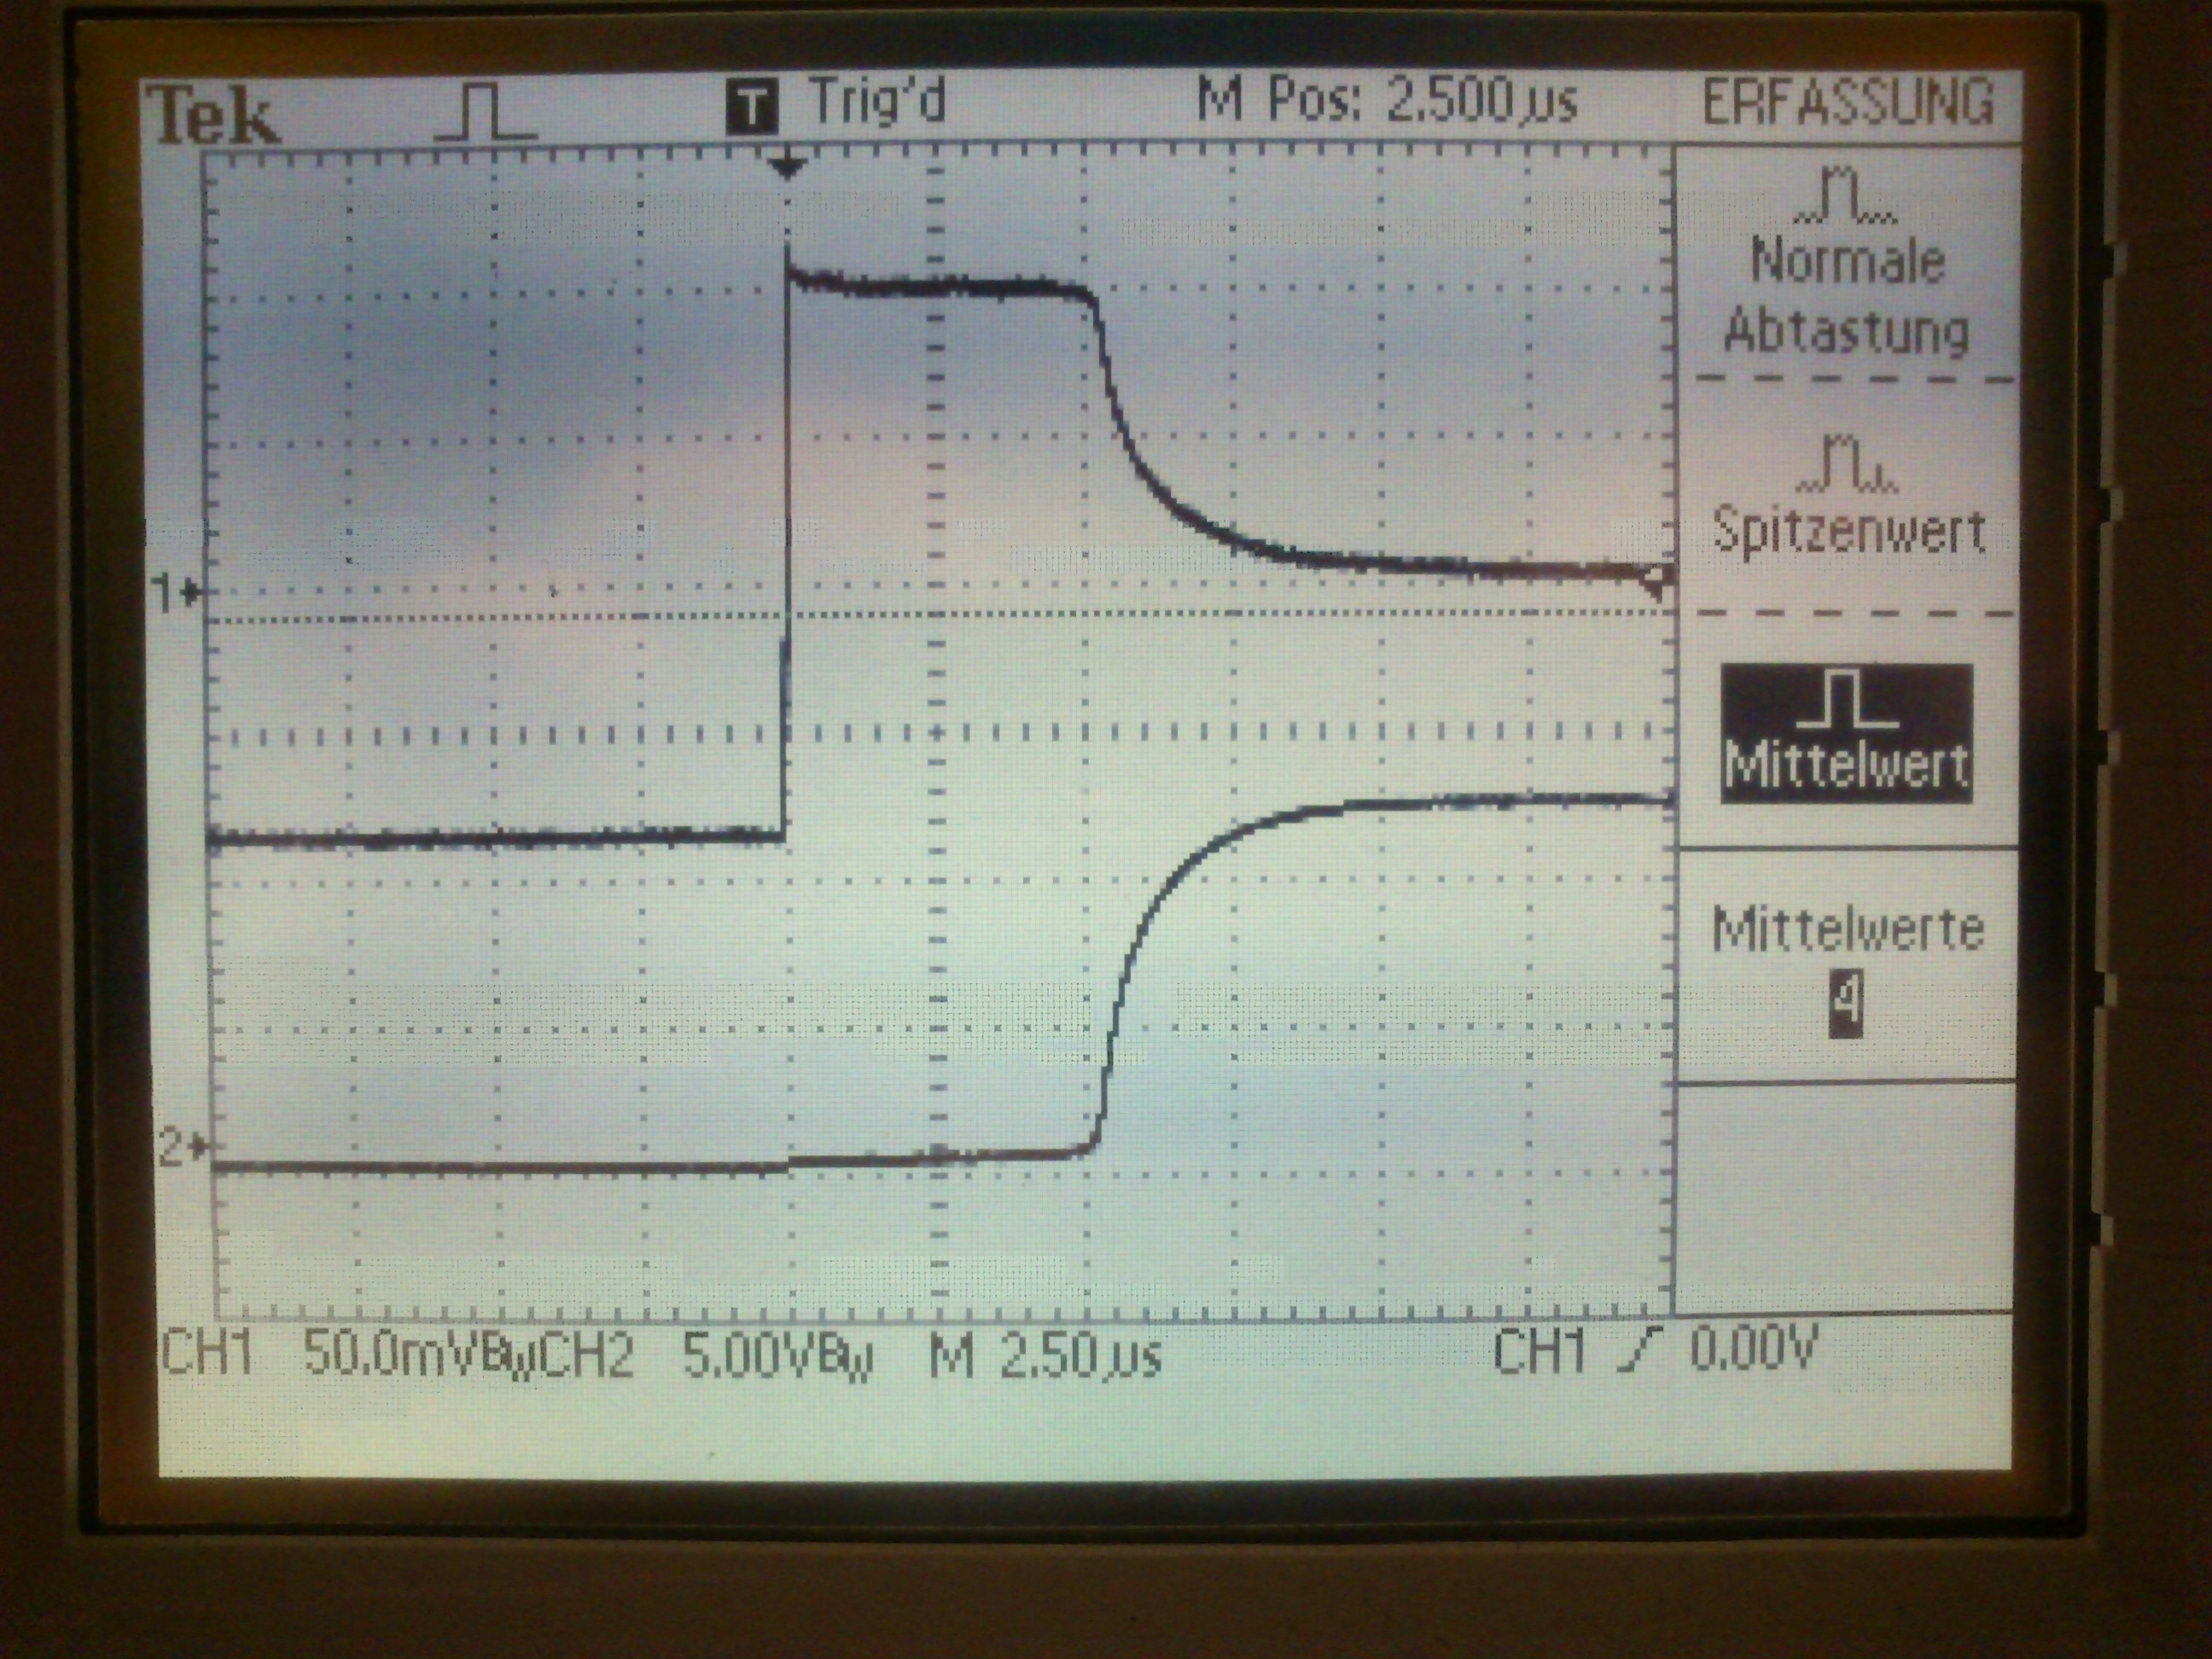
\includegraphics[width=\linewidth]{versuch2/oszi/DSC_0230.JPG}
	\caption{Messung der Speicherzeit}
\end{figure}
Spannend ist, dass der Strom in Sperrrichtung kurzzeitig größer ist, als der in Durchlassrichtung. Dies rührt daher, dass in der Diode noch freie Ladungsträger sind, die zusätzlich zum angelegten Strom abfließen während die Sperrschicht aufgebaut wird.\\
Durch ihre lange Speicherzeit ist diese Diode für höhere Frequenzen nicht geeignet, weil sie dann einfach durchgehend leiten würde. In einem Schaltnetzteil würde sie einfach garnicht mehr schalten, sondern dauerhaft leiten.\\
Die lange Speicherzeit rührt wahrscheinlich von der dicken Sperrschicht her, die diese Diode braucht. Immerhin hält sie 1000 V Sperrspannung aus.
%}}}

%{{{
\subsection{Sample-Hold-Schaltung}
In Spice wurde eine Sample-And-Hold-Schaltung aufgebaut und simuliert:
\begin{figure}[H]
	\centering
	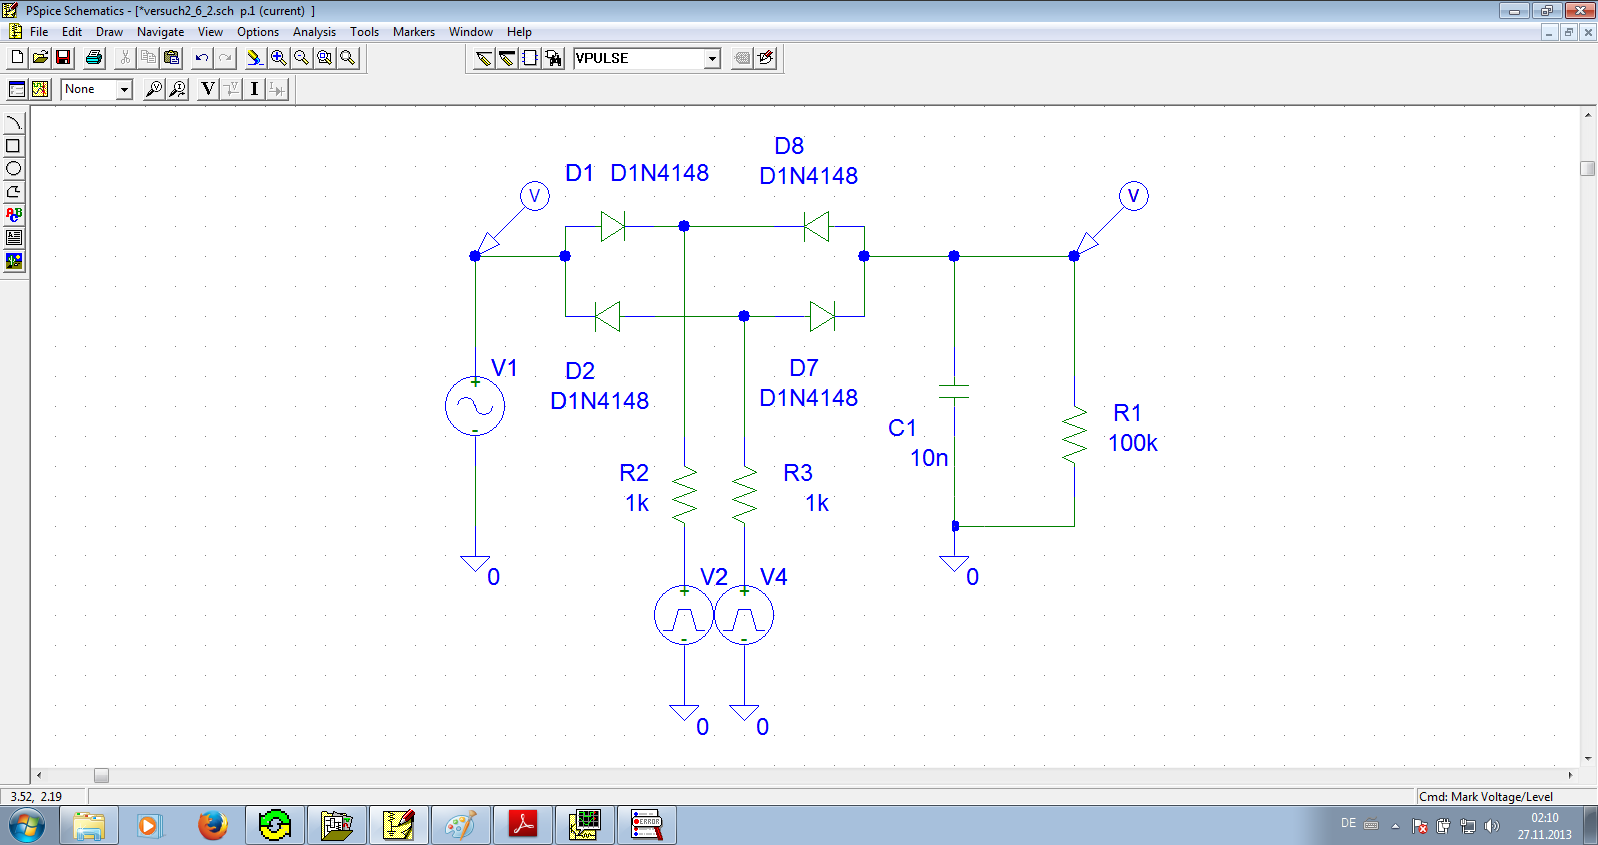
\includegraphics[width=\linewidth]{versuch2/spice/v2_8_1_schematic.png}
	\caption{Schaltplan für die Simulation mit Pspice}
\end{figure}
Das ergab simuliert:
\begin{figure}[H]
	\centering
	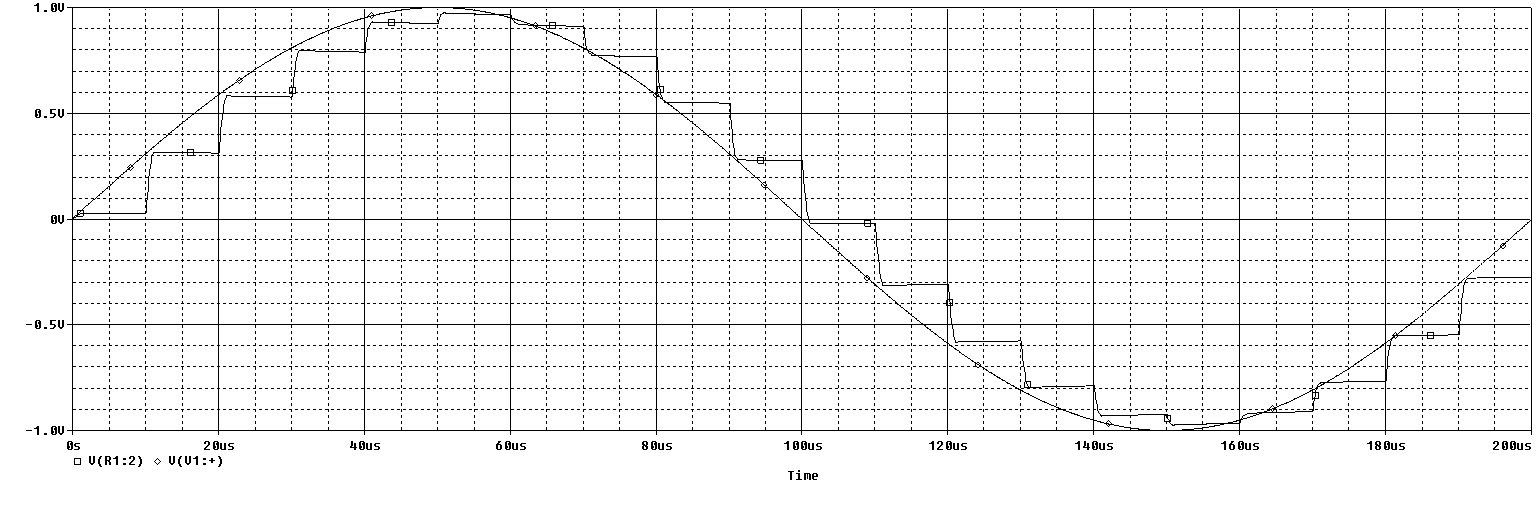
\includegraphics[width=\linewidth]{versuch2/spice/v2_8_1_simulation.png}
	\caption{Und die Simulationsergebnisse}
\end{figure}
Die Schaltung nimmt während eines Impules der Impulsspannungsquellen die Spannung der Sinunsspannungsquelle und speichert ihren Wert im nachgeschalteten Kondensator ab.\\
Der Trick liegt dabei darin, dass die beiden Dioden durch ihre Speicherzeit ähnlich wie ein Transistor genutzt werden. Durch die extrem scharfe Flanke der Puls-Signalquellen werden die Dioden in Sperrichtung leitend und verbinden so den nachgeschalteten Schaltkreis mit der Spannungsquelle. Und nach dem Ende der Speicherzeit sind sind die Dioden wieder sperrend und trennen so die Schaltung von der Spannungsquelle ab. Damit die Schaltung gut funktionieren kann, sind möglichst scharfe Flanken bei der Beschaltung der Dioden unerlässlich. Alternativ kann man Dioden mit längerer Speicherzeit verwenden, dann bekommen man aber kein sauberes Sampling mehr.
%}}}

%}}}
